\documentclass[17pt, t, lualatex]{beamer}



\title{Hidrodinámica fluvial en el río Magdalena en Barrancabermeja: Un modelo accesible para simular ríos}
\date{\today}
\institute[UJTL]{Universidad Jorge Tadeo Lozano}
\author{Ludwig Alvarado Becerra}

\usepackage{amsmath, amssymb, mathtools}
\usepackage{graphicx}
\usepackage[spanish]{babel}
\usepackage{biblatex}
\usepackage{hyperref}
\usepackage{xurl}
\usepackage{svg}
\usepackage{listings}
\usepackage[scale=7]{ccicons}


\addbibresource{referencias.bib}  % Make sure your .bib file is correctly named


\addbibresource{referencias.bib}


\definecolor{white}{HTML}{FFFFFF}
\definecolor{sand}{HTML}{EBE5E0}
\definecolor{KTHblue}{HTML}{004791}
\definecolor{skyblue}{HTML}{6298D2}
\definecolor{navy}{HTML}{000061}
\definecolor{lightblue}{HTML}{DEF0FF}
\definecolor{digitalblue}{HTML}{0029ED}


\lstset{
  language=bash,                       % Set the language to bash
  backgroundcolor=\color{white},       % Background color for the code block
  basicstyle=\ttfamily\normalsize,    % Use typewriter font and small size
  keywordstyle=\color{KTHblue},           % Style for keywords (e.g. if, for, etc.)
  commentstyle=\color{sand},          % Style for comments
  stringstyle=\color{skyblue},             % Style for strings
  showstringspaces=false,              % Don't underline spaces in strings
  breaklines=true,                     % Automatically break long lines
  frame=single,                        % Add a frame around the code
  captionpos=b,                        % Position of the caption (bottom)
  numbers=left,                        % Line numbers on the left
  numberstyle=\tiny\color{gray},       % Style for line numbers
  stepnumber=1,                        % Display every line number
  numbersep=5pt,                       % Space between line numbers and code
  morekeywords={bat, wc, tail, cut, head, >},
}



% Probably load as late as possible
% Other options are
% - engine=pdflatex to compile in pdfLaTeX (with different fonts),
% - mathshape=rm to use serif font for math,
% - mathsahpe=custom to not set any math font (so that you can define your own math fonts)
\usetheme[engine=lualatex, mathshape=sf, fontdir=kthpq-files/fonts/Figtree/]{kthpq}
\setmonofont{Bitstream Vera Sans Mono}[Scale=.9]

% Custom colors (see beamercolorthemecustom.sty for more details)
% \usecolortheme{custom}

% Modify the headline template: KTH-full, KTH-section-only, or KTH-frametitle-only.
% \setbeamertemplate{headline}[KTH-full]

% Custom footline
% \setfootline{left}{center}{right}



\begin{document}

\inserttitlepage

\section{Problema}

\insertsectionpage

\begin{frame}[allowframebreaks]
  \frametitle{Problema}

  \begin{columns}
    \begin{column}{.5\textwidth}
      \begin{itemize}
        \item Actualmente estamos en un período de lluvias fuerte, generalmente, significa un aumento en el caudal.
        \item Modelar de manera correcta cómo se comporta un río a lo largo del tiempo es importante para la prevención de futuros desastres que perjudiquen a la población.
      \end{itemize}
    \end{column}

    \begin{column}{.5\textwidth}
      \begin{figure}[ht]
        \centering
        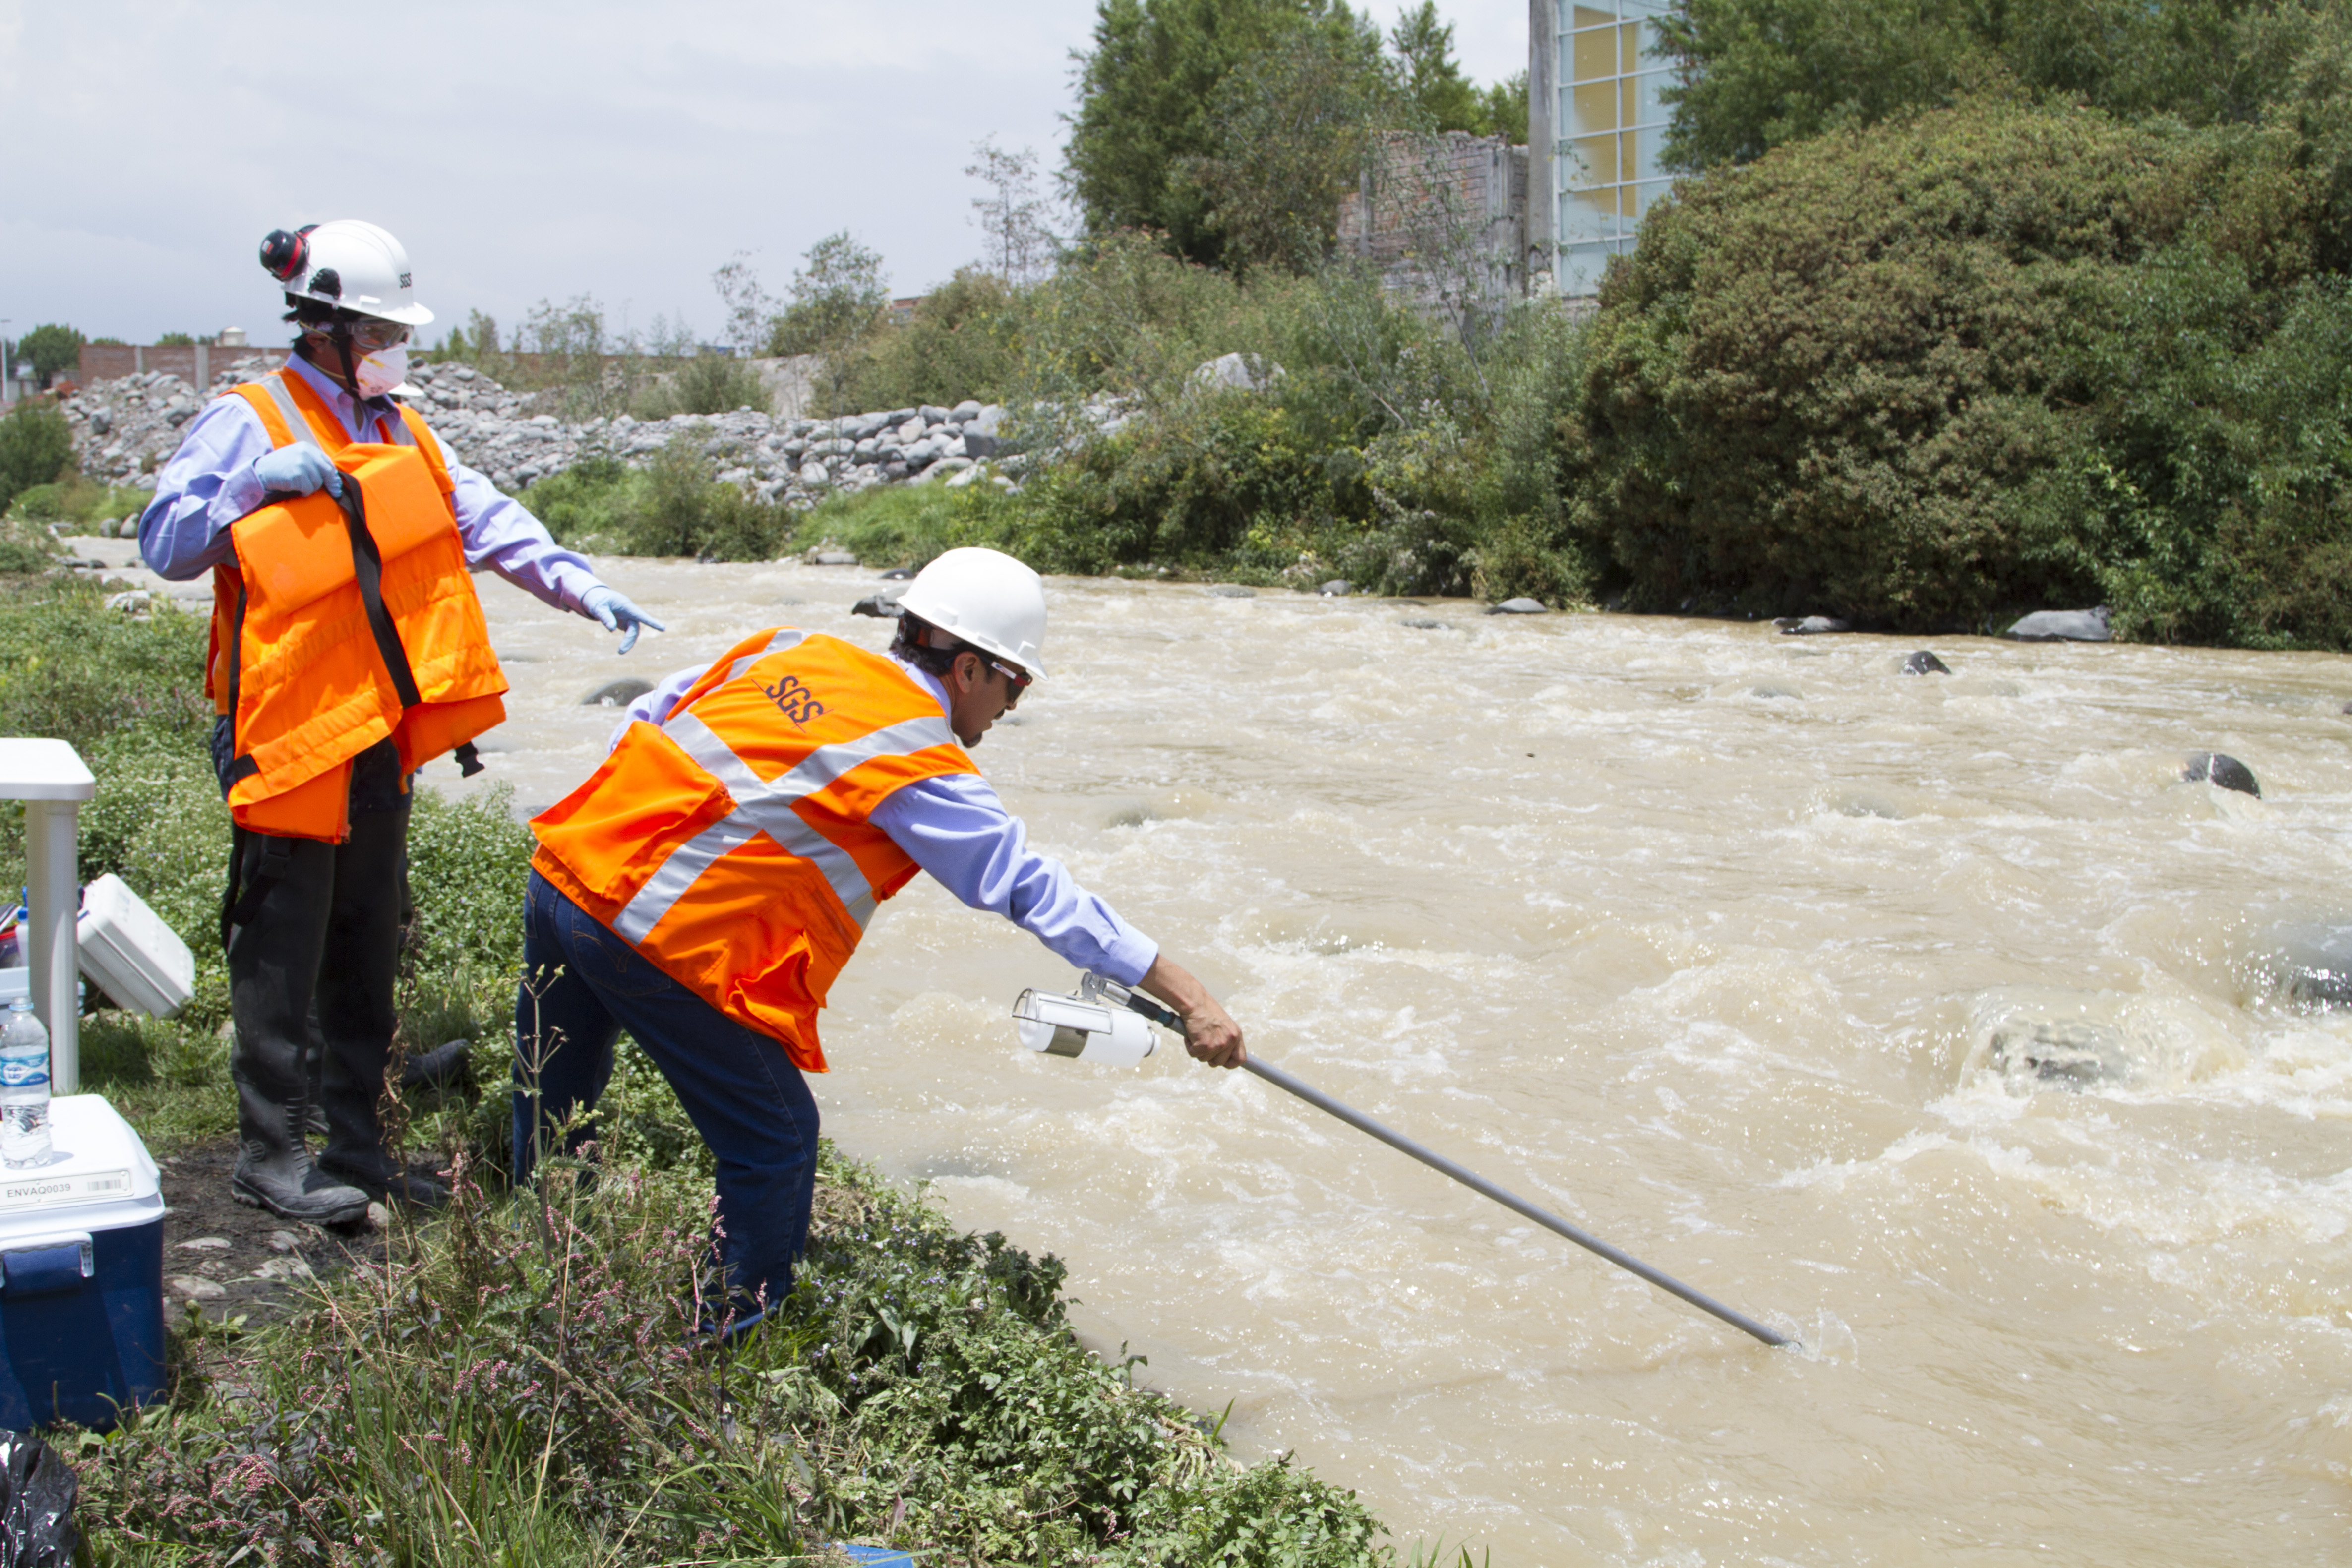
\includegraphics[width=\textwidth]{img/Caudal1.jpg}
      \end{figure}

    \end{column}
  \end{columns}

\end{frame}



\section{Objetivos}

\insertsectionpage

\begin{frame}[allowframebreaks]
  \frametitle{Objetivos}

  \begin{columns}
    \begin{column}{.5\textwidth}
      \begin{itemize}
        \item Desarrollar una herramienta que permita realizar simulaciones sobre la dinámica de un río dado unos datos enviados por el usuario.
        \item Aplicar un modelo matemático que modele la situación del caudal y el área transversal de una región del río.
        \item Desplegar el modelo para que pueda ser utilizado y replicado por cualquier persona con conexión a internet.
    \end{itemize}
    \end{column}

    \begin{column}{.5\textwidth}
      \begin{figure}[ht]
        \centering
        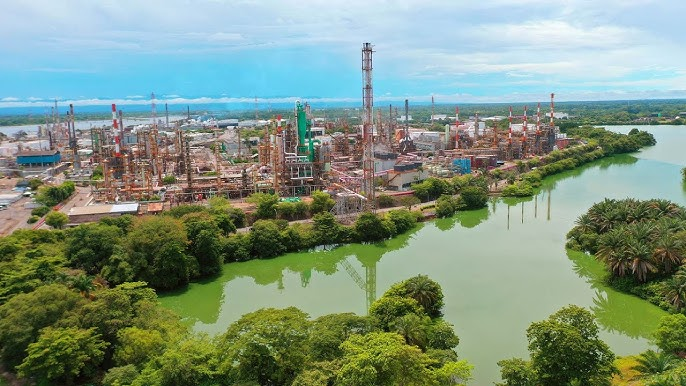
\includegraphics[width=\textwidth]{img/Rio1.jpg}
        \caption{Rio Magdalena a la altura de Barrancabermeja}
      \end{figure}

    \end{column}
  \end{columns}

\end{frame}


\begin{frame}[plain]
\frametitle{}  % no title
\begin{figure}[ht]
  \centering
  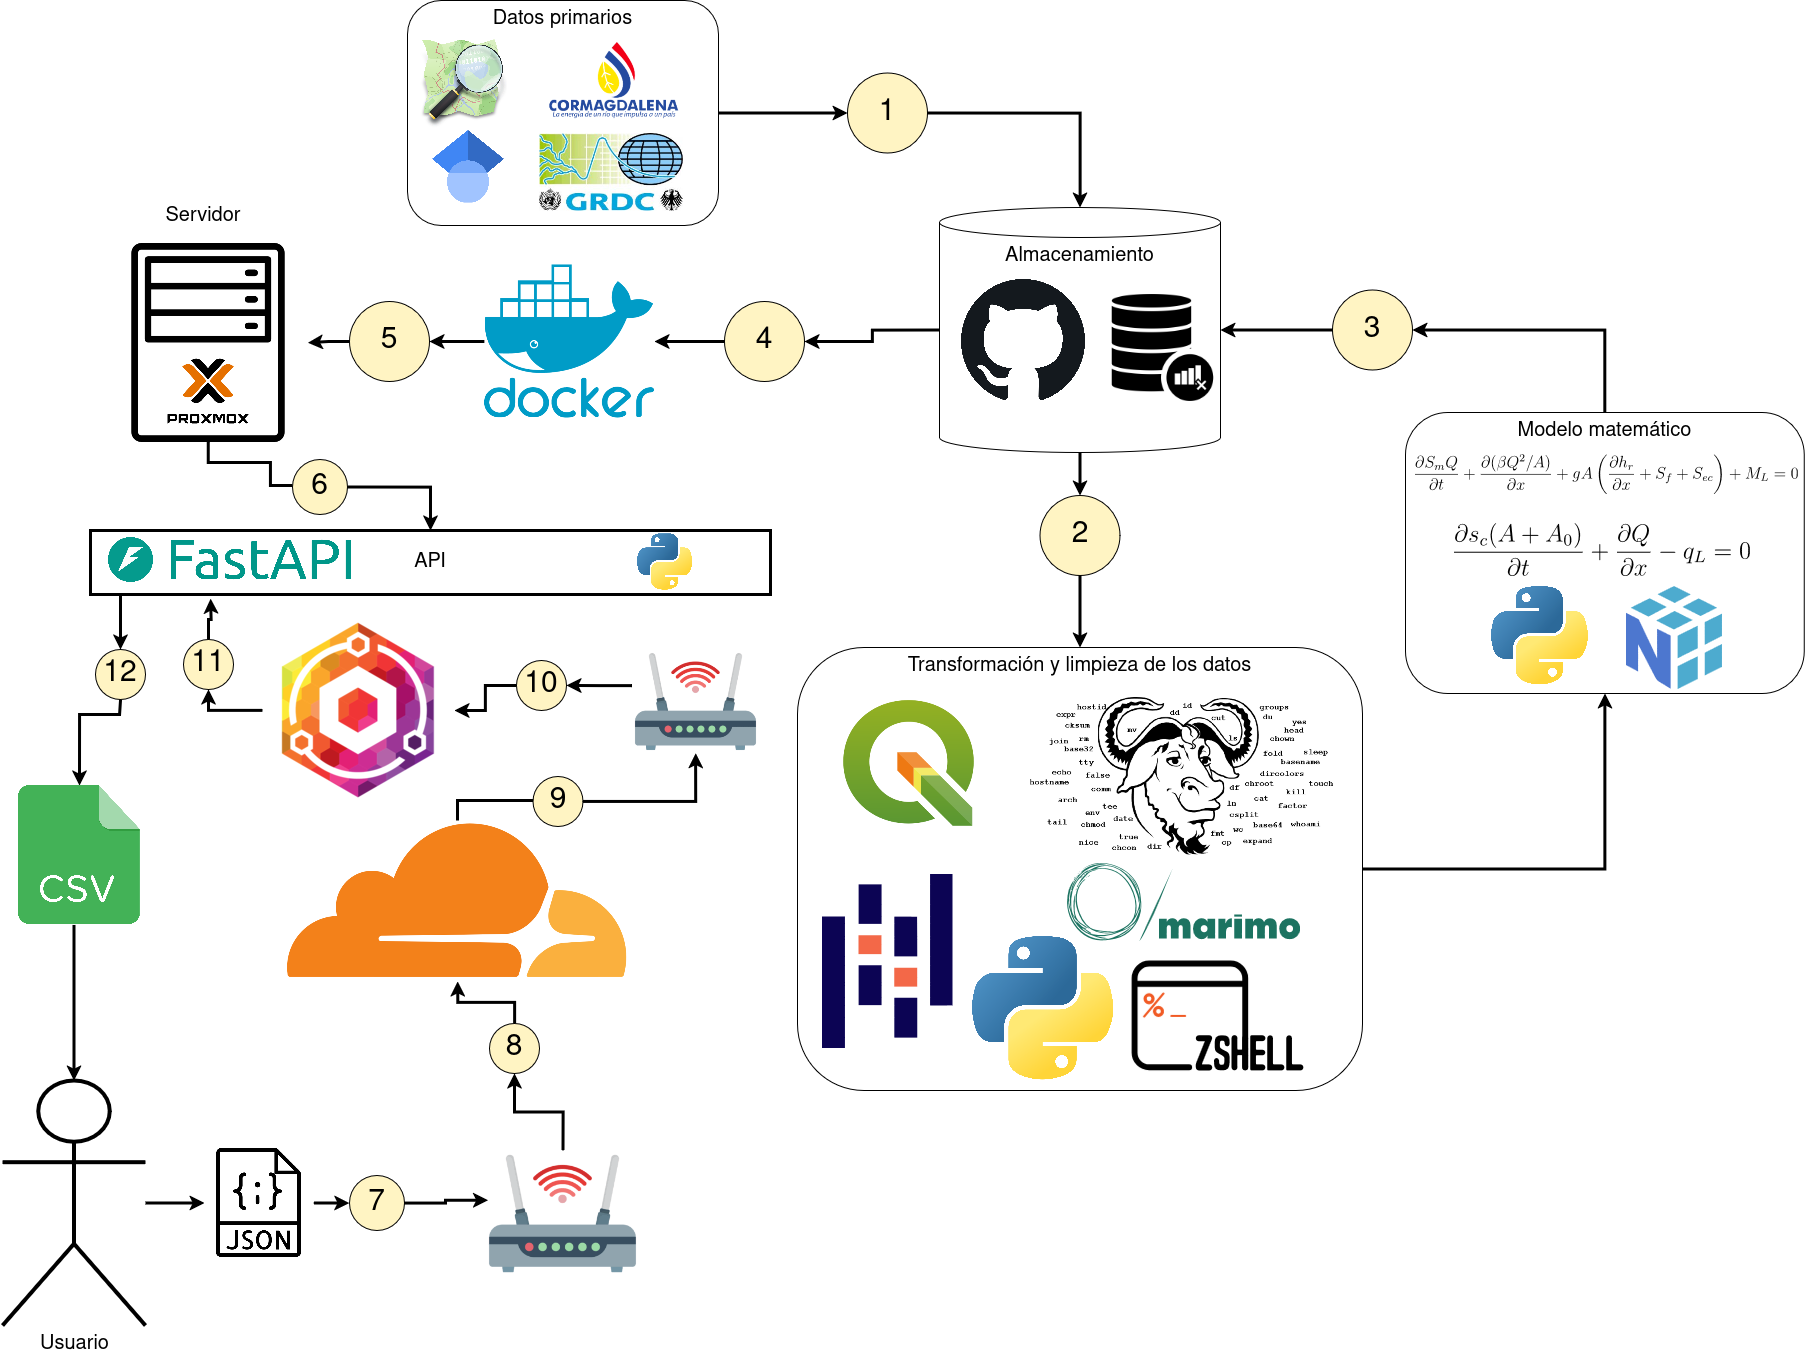
\includegraphics[width=0.8\textwidth]{img/Arquitectura.png}
\end{figure}

\end{frame}


\section{Datos necesarios}

\insertsectionpage

\begin{frame}[allowframebreaks]
  \frametitle{Datos necesarios}

  \begin{itemize}
    \item Coeficiente de rugosidad de Manning\cite{garcia2020mathematical}. 
    \item Dimensiones del río de ancho y largo.
    \item Pendiente del río.  
    \item Limpieza de duplicados con los datos de la elevación del río.
    \item Limpieza general de datos del caudal del río.
    \item Condiciones iniciales y finales.
    \item Implementación en código del modelo.
  \end{itemize}

\end{frame}



\section{Región de estudio}

\insertsectionpage

\begin{frame}[allowframebreaks]
  \frametitle{Región de estudio}
  
  \begin{figure}[ht]
    \centering
    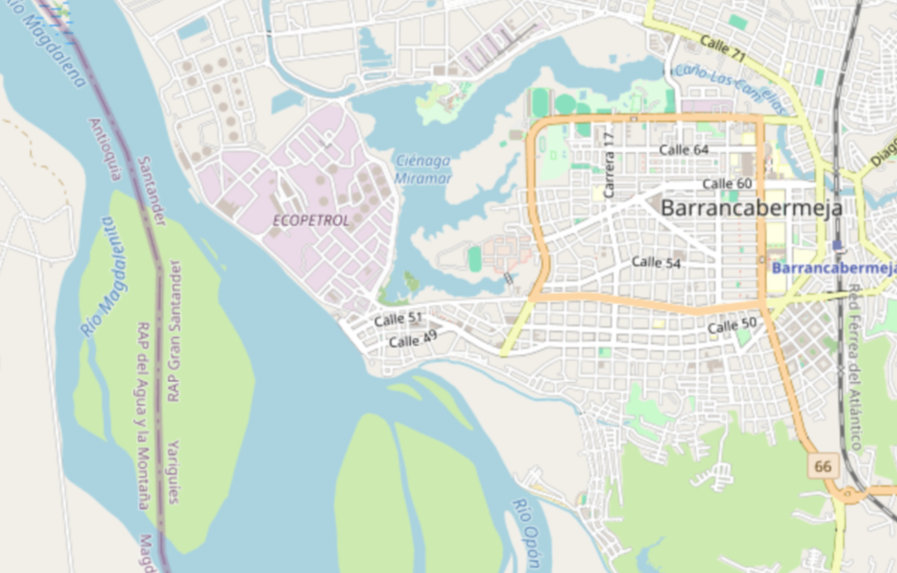
\includegraphics[width=0.5\textwidth]{img/OSM-1.png}
    \caption{Región a estudiar del Río Magdalena. Datos de \textit{OpenStreetMap} (OSM)\cite{openstreetmap_magdalena2025}}
  \end{figure}

  \begin{figure}[ht]
    \centering
    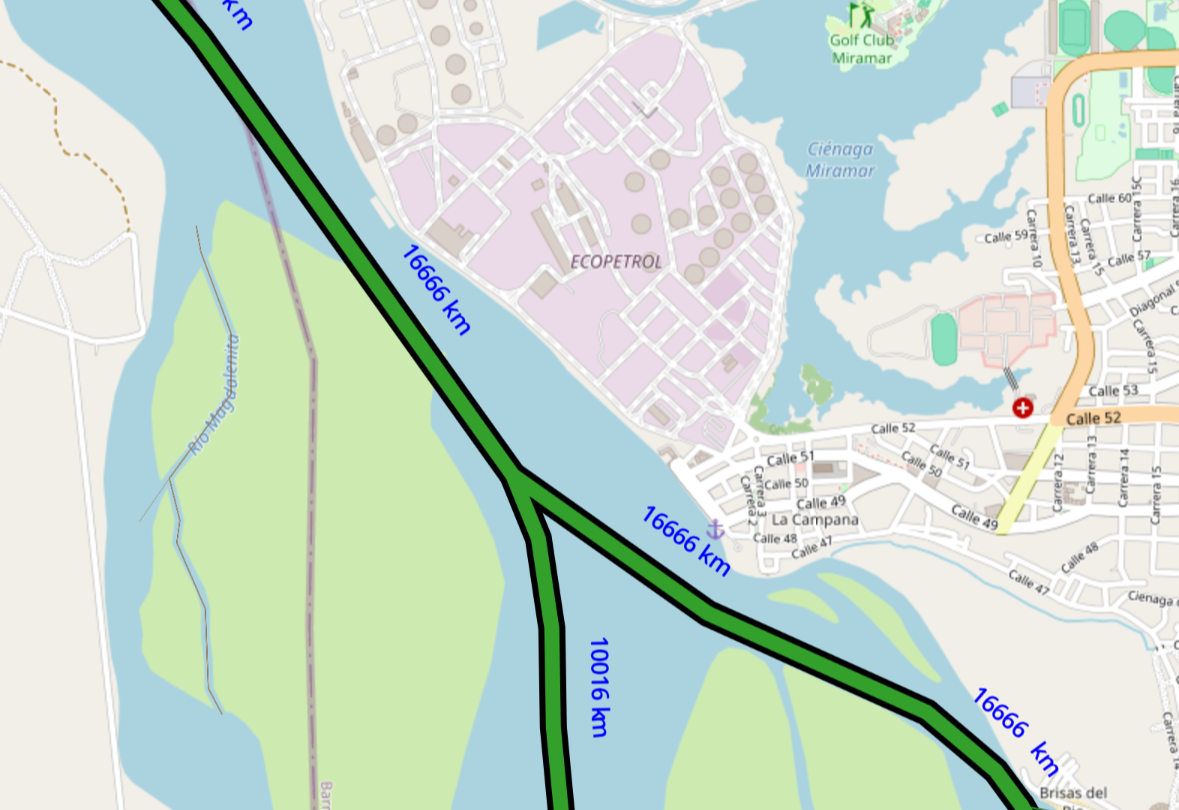
\includegraphics[width=0.5\textwidth]{img/Waterway.png}
    \caption{Río Magdalena. Datos sacados de \textit{Waterway}\cite{waterwaymap2025}}
  \end{figure}

  \begin{figure}[ht]
    \centering
    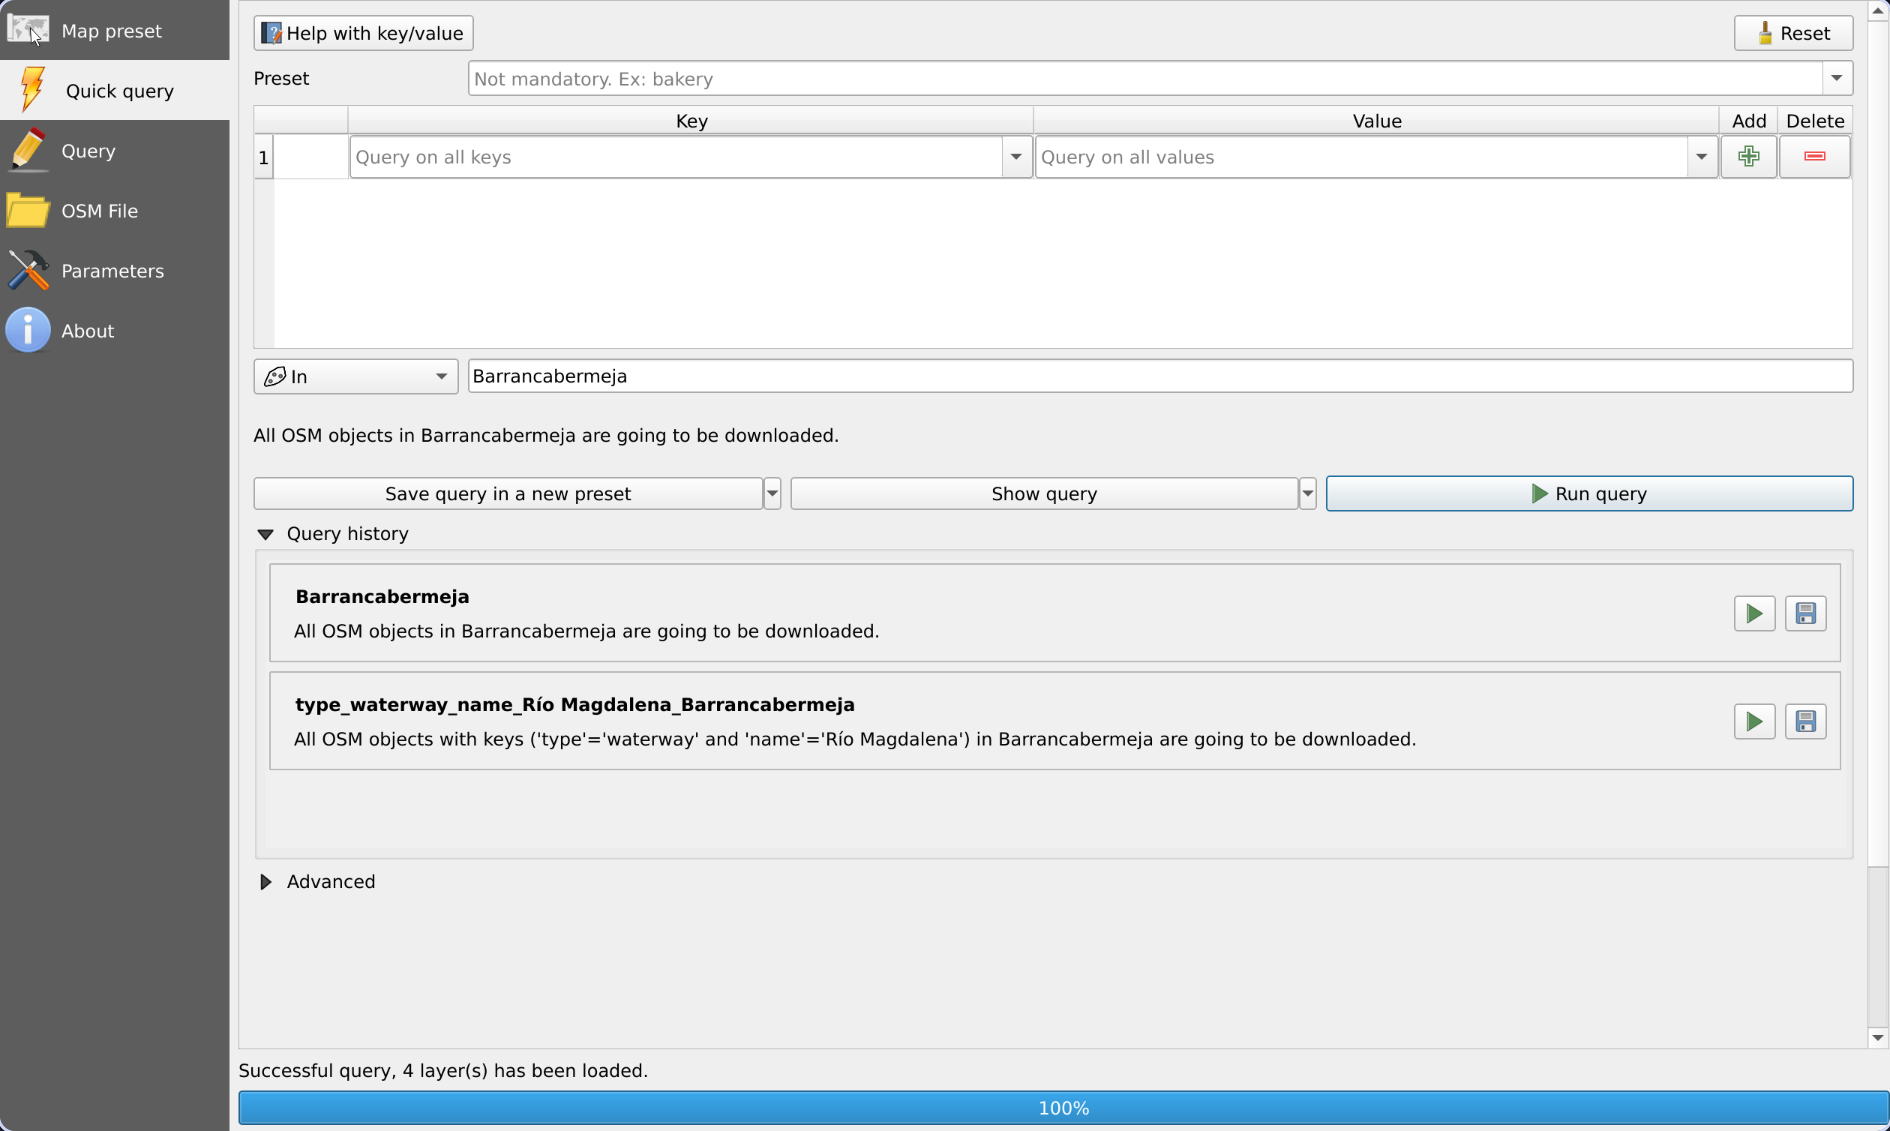
\includegraphics[width=0.5\textwidth]{img/QGIS-5.png}
    \caption{Consulta de datos utilizando QuickOSM\cite{quickosm2025}}
  \end{figure}


  \begin{figure}[ht]
    \centering
    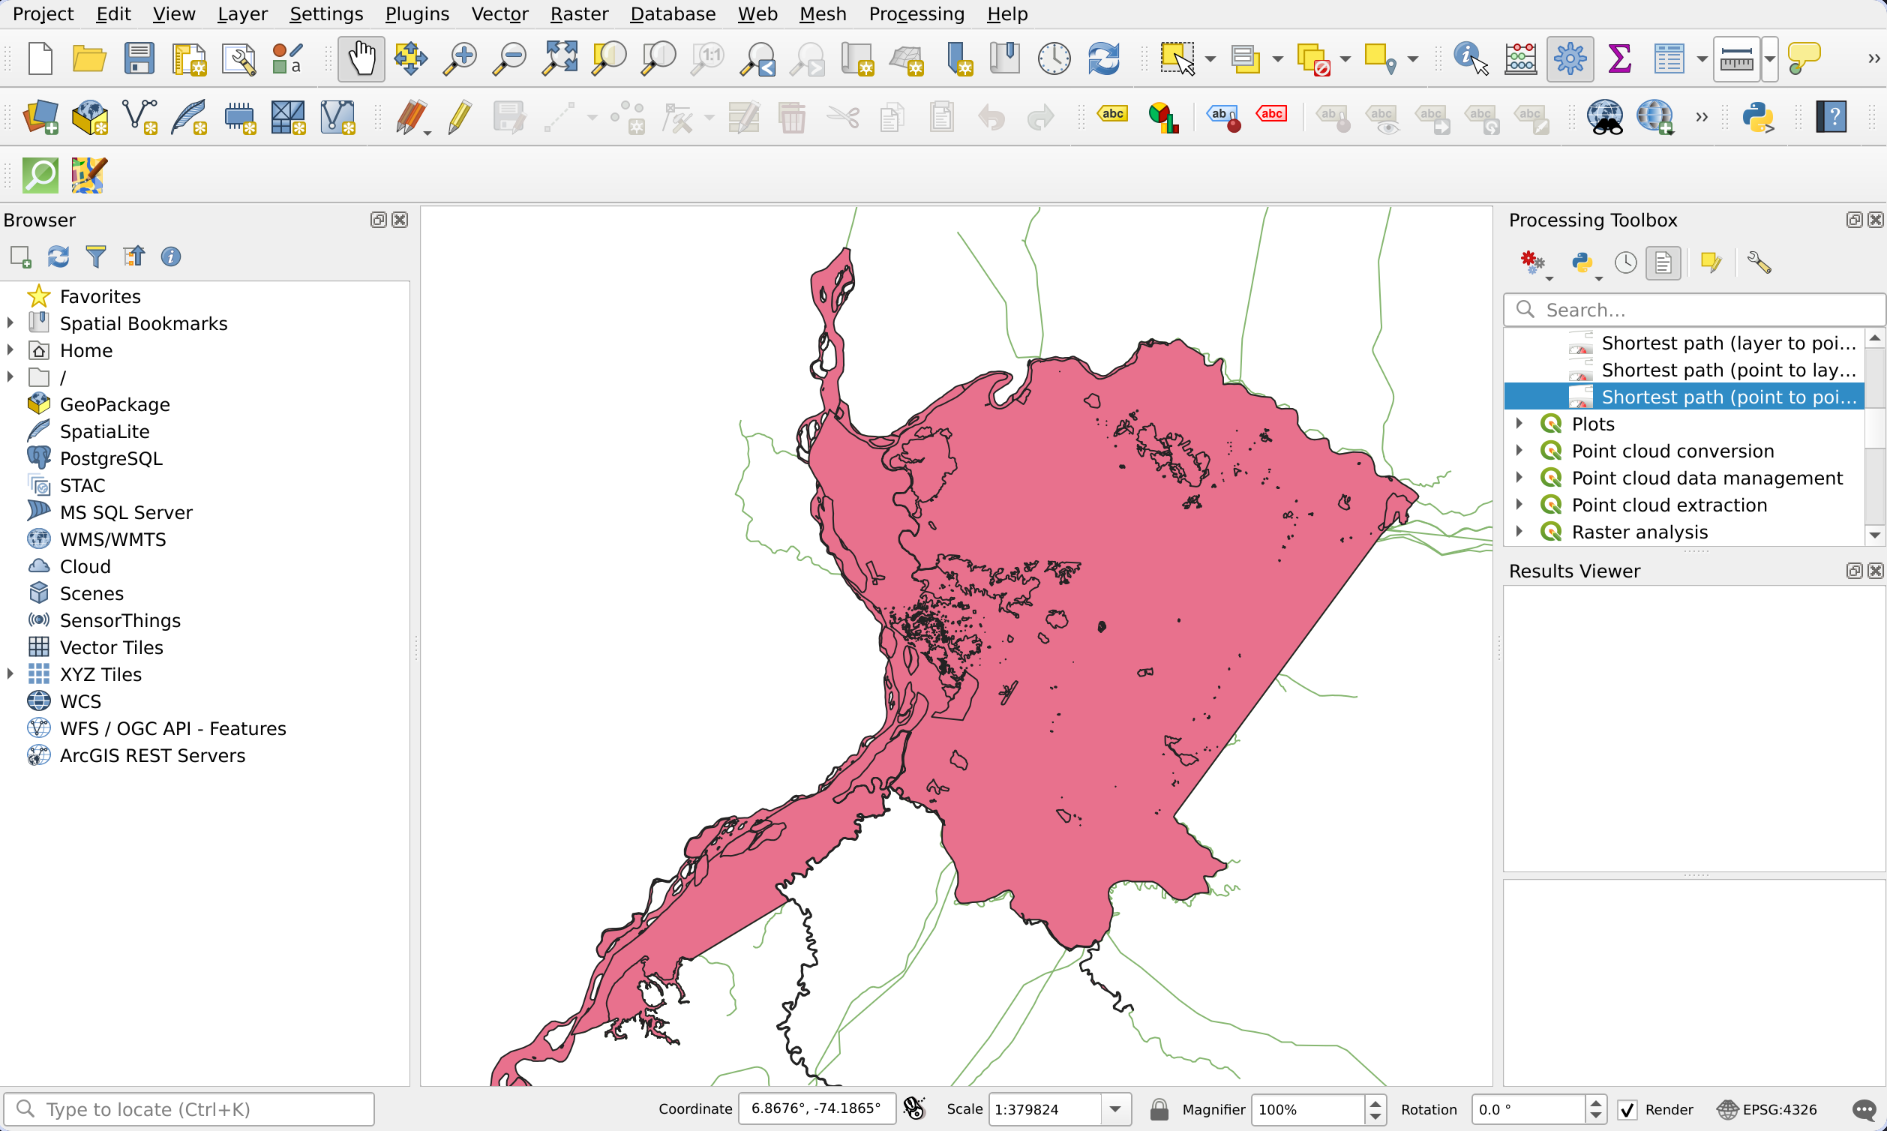
\includegraphics[width=0.55\textwidth]{img/QGIS-1.png}
    \caption{Región de Barrancabermeja, elaboración propia en QGIS\cite{qgis2025}, datos de OSM\cite{openstreetmap_magdalena2025}.}
  \end{figure}


  \begin{columns}
    \begin{column}{.3\textwidth}
      \begin{itemize}
        \item Se filtra la capa del Río Magdalena y se le cambia el color para que destaque.
      \end{itemize}
    \end{column}

    \begin{column}{.7\textwidth}
      \begin{figure}[ht]
        \centering
        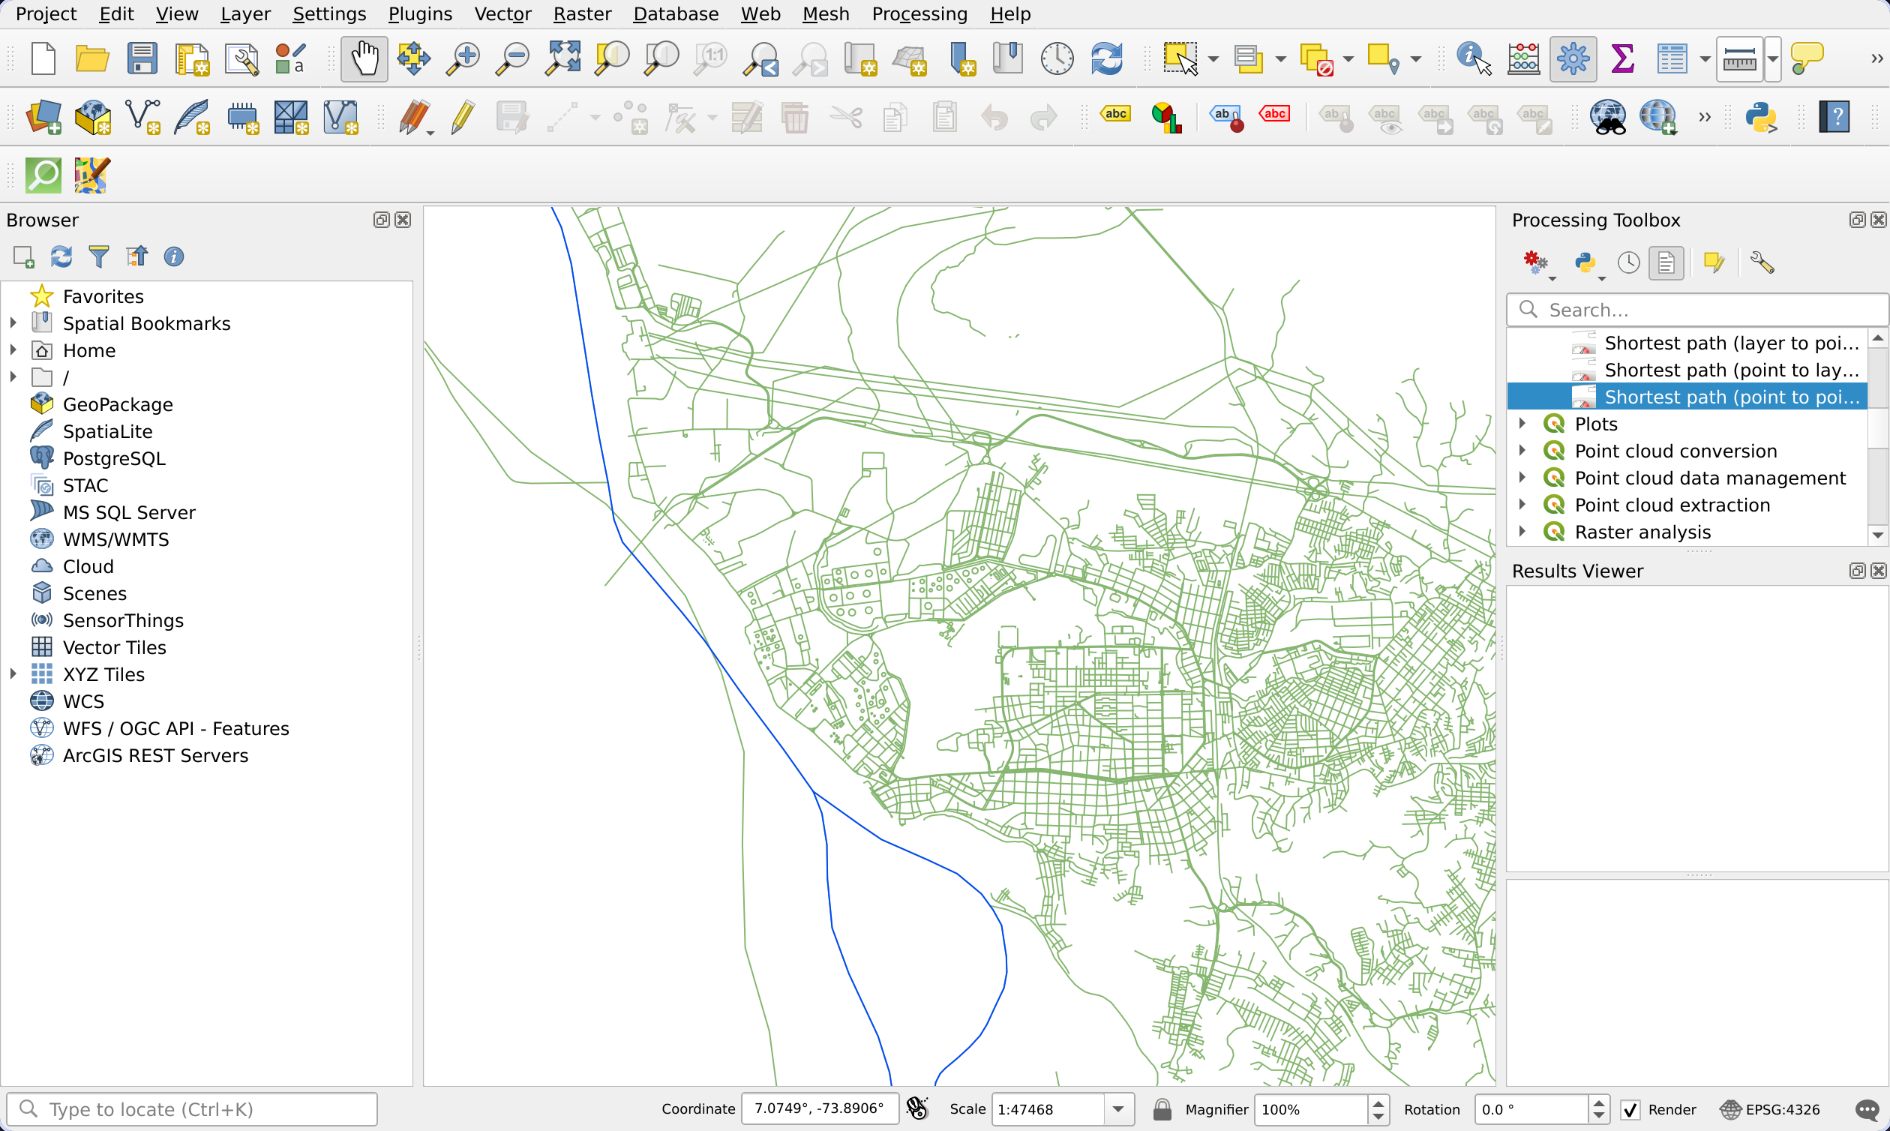
\includegraphics[width=0.8\textwidth]{img/QGIS-2.png}
        \caption{Elaboración propia.}
      \end{figure}
    \end{column}
  \end{columns}


  \begin{columns}
    \begin{column}{.3\textwidth}
      \begin{itemize}
        \item Utilizar \texttt{Vector} > \texttt{Geometry Tools} > \texttt{Extract Vertices...}
      \end{itemize}
    \end{column}

    \begin{column}{.7\textwidth}
      \begin{figure}[ht]
        \centering
        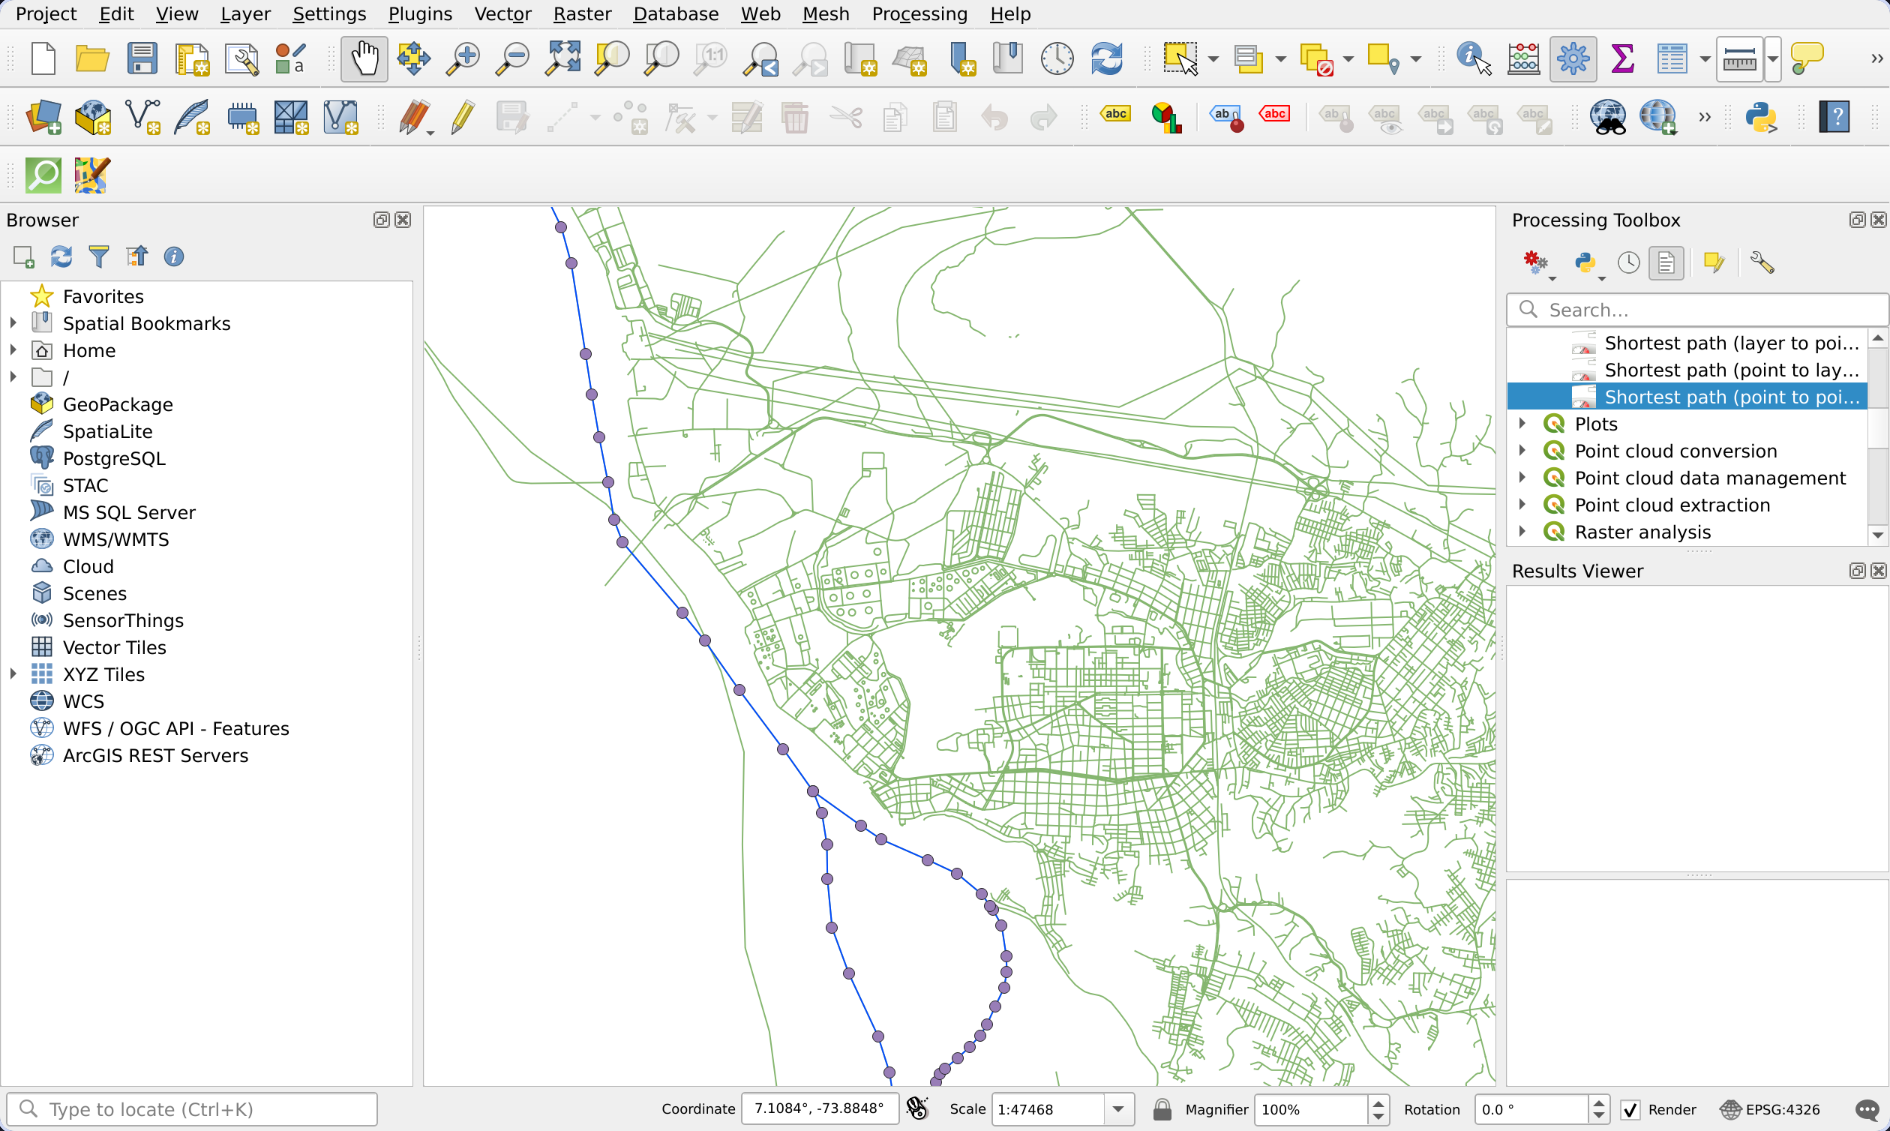
\includegraphics[width=0.8\textwidth]{img/QGIS-3.png}
        \caption{Elaboración propia.}
      \end{figure}
    \end{column}
  \end{columns}

  \begin{columns}
    \begin{column}{.3\textwidth}
      \begin{itemize}
        \item Se seleccionan el segmento que se de interés para el estudio. 
      \end{itemize}
    \end{column}

    \begin{column}{.7\textwidth}
      \begin{figure}[ht]
        \centering
        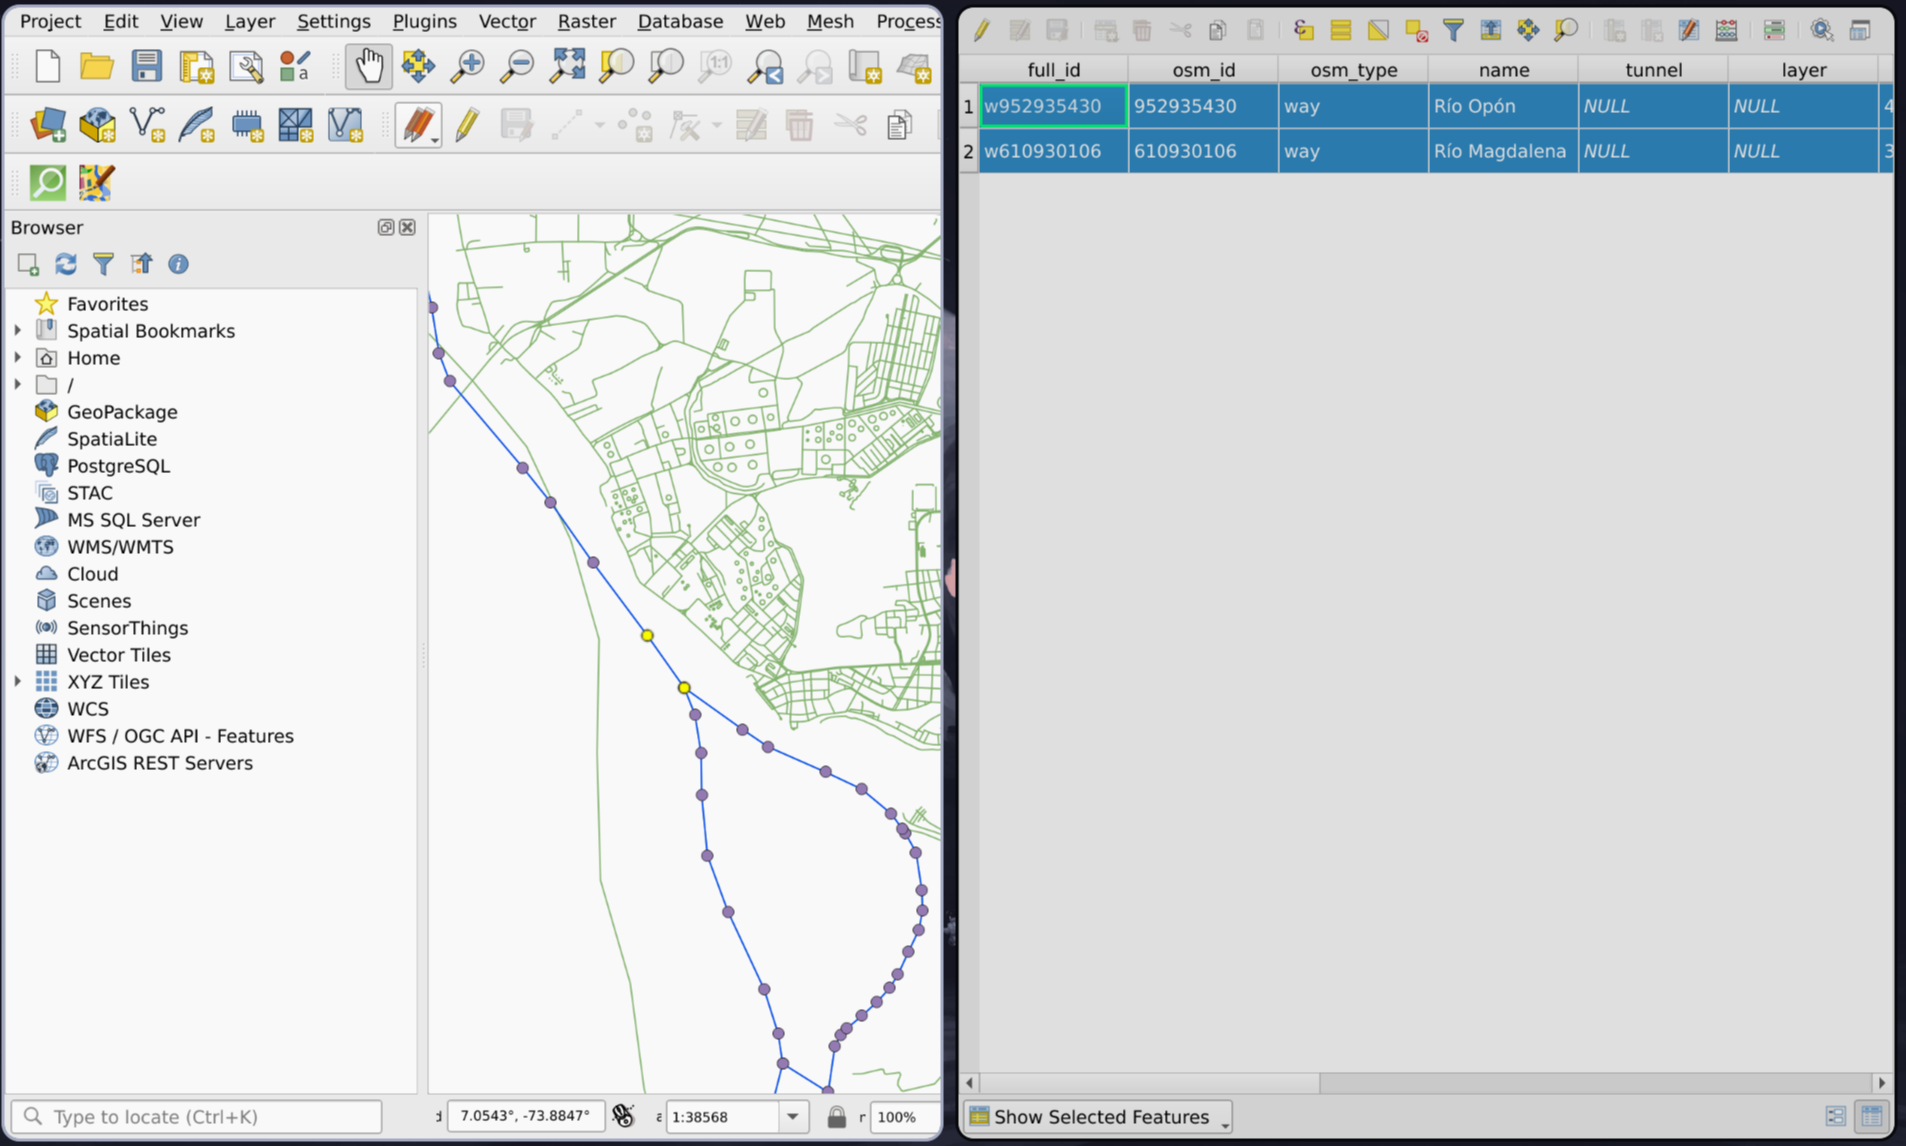
\includegraphics[width=0.8\textwidth]{img/QGIS-4.png}
        \caption{Elaboración propia.}
      \end{figure}
    \end{column}
  \end{columns}

  \begin{columns}
    \begin{column}{.3\textwidth}
      \begin{itemize}
        \item Utilizando la herramienta de \texttt{Distance matrix...} se obtienen $472.7434 \text{ metros}$ .
      \end{itemize}
    \end{column}

    \begin{column}{.7\textwidth}
      \begin{figure}[ht]
        \centering
        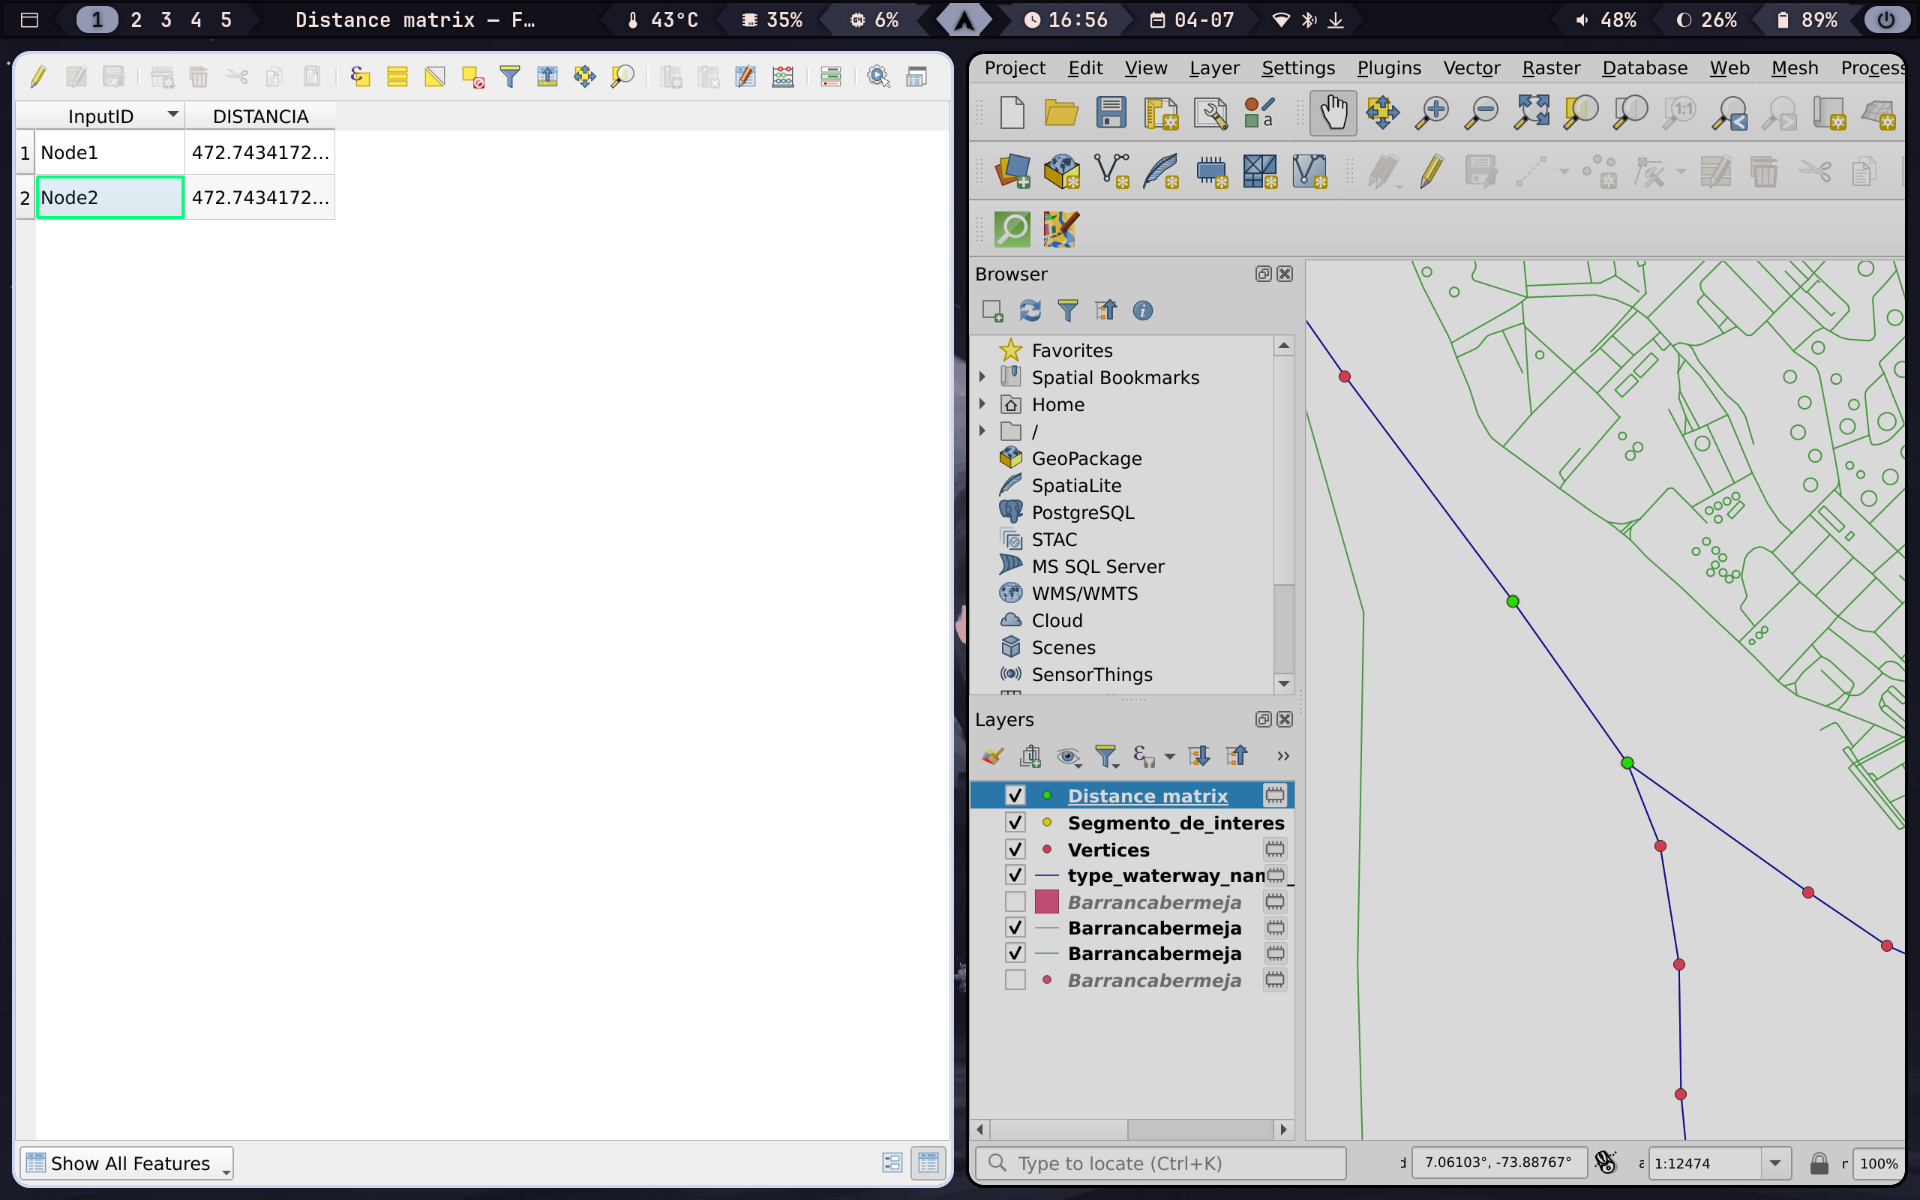
\includegraphics[width=0.7\textwidth]{img/QGIS-6.png}
        \caption{Elaboración propia.}
      \end{figure}
    \end{column}
  \end{columns}

\end{frame}





\begin{frame}
  \frametitle{Consulta del ancho}

  \begin{columns}
    \begin{column}{.3\textwidth}
      \begin{itemize}
        \item Usando la opción \texttt{Open Field Calculator} se puede consultar la información de estos datos como si fuera SQL.
        \item El resultado de esto son $300 \text{ metros}$
      \end{itemize}
    \end{column}

    \begin{column}{.7\textwidth}
      \begin{figure}[ht]
        \centering
        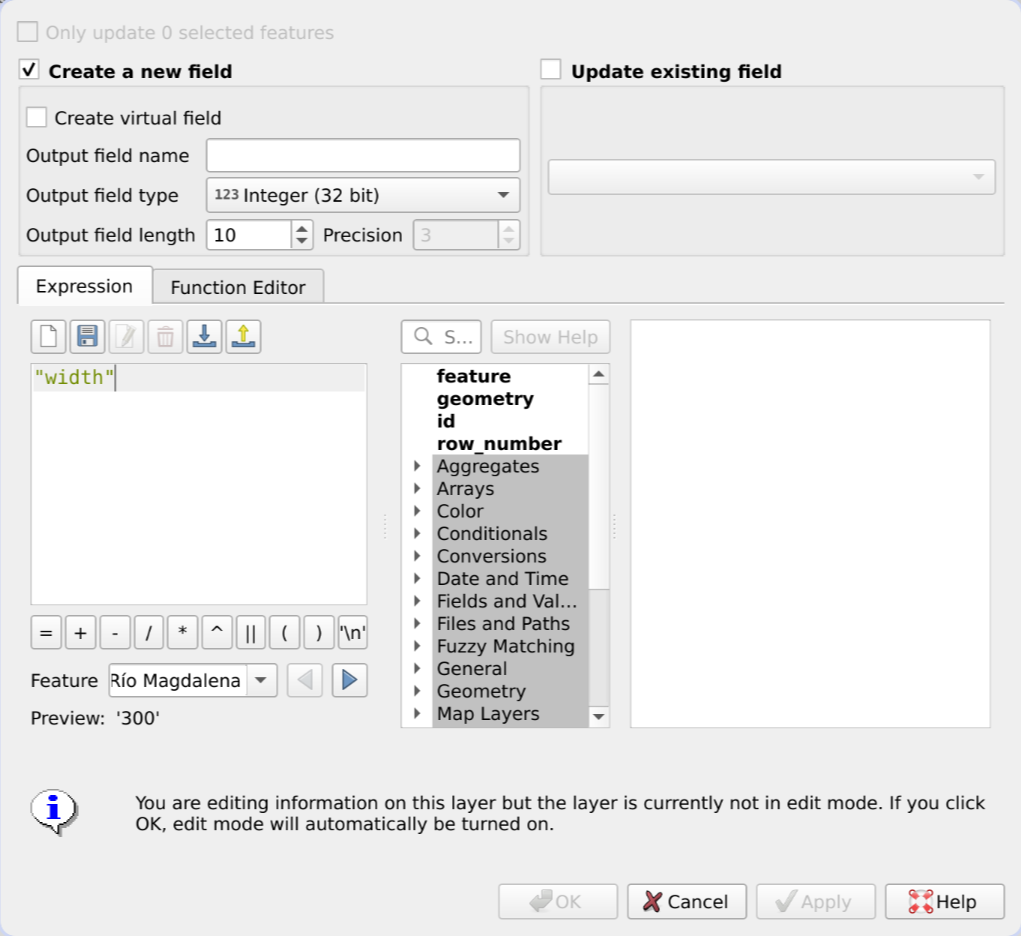
\includegraphics[width=0.5\textwidth]{img/QGIS-7.png}
        \caption{Consulta del ancho del Río Magdalena.}
      \end{figure}
    \end{column}
  \end{columns}

\end{frame}

\begin{frame}
  \frametitle{Coeficiente de rugosidad y pendientes}

  \begin{columns}
    \begin{column}{.3\textwidth}
      \begin{itemize}
        \item Coeficiente de Mannig: $0.018$
        \item Pendiente del río: $0.07\%$
      \end{itemize}
    \end{column}

    \begin{column}{.7\textwidth}
      \begin{figure}[ht]
        \centering
        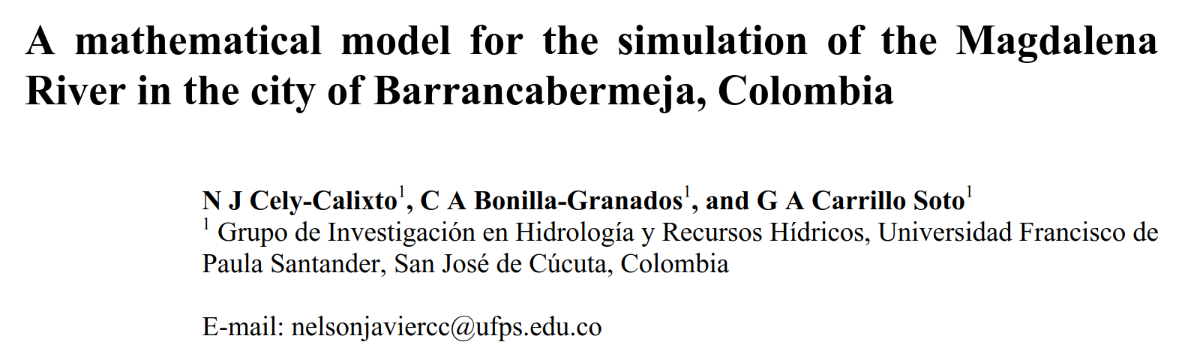
\includegraphics[width=1\textwidth]{img/Paper.png}
        \caption{\textit{A mathematical model for the simulation of the Magdalena River in the city of Barrancabermeja, Colombia}\cite{garcia2020mathematical}.}
      \end{figure}
    \end{column}
  \end{columns}

\end{frame}





\begin{frame}
  \frametitle{Elevación del río}

  \begin{columns}
    \begin{column}{.3\textwidth}
      \begin{itemize}
        \item Script en \textit{Python} utilizando web scrapping con BeautifulSoup
        \item Datos desordenados.
      \end{itemize}
    \end{column}

    \begin{column}{.7\textwidth}
      \begin{figure}[ht]
        \centering
        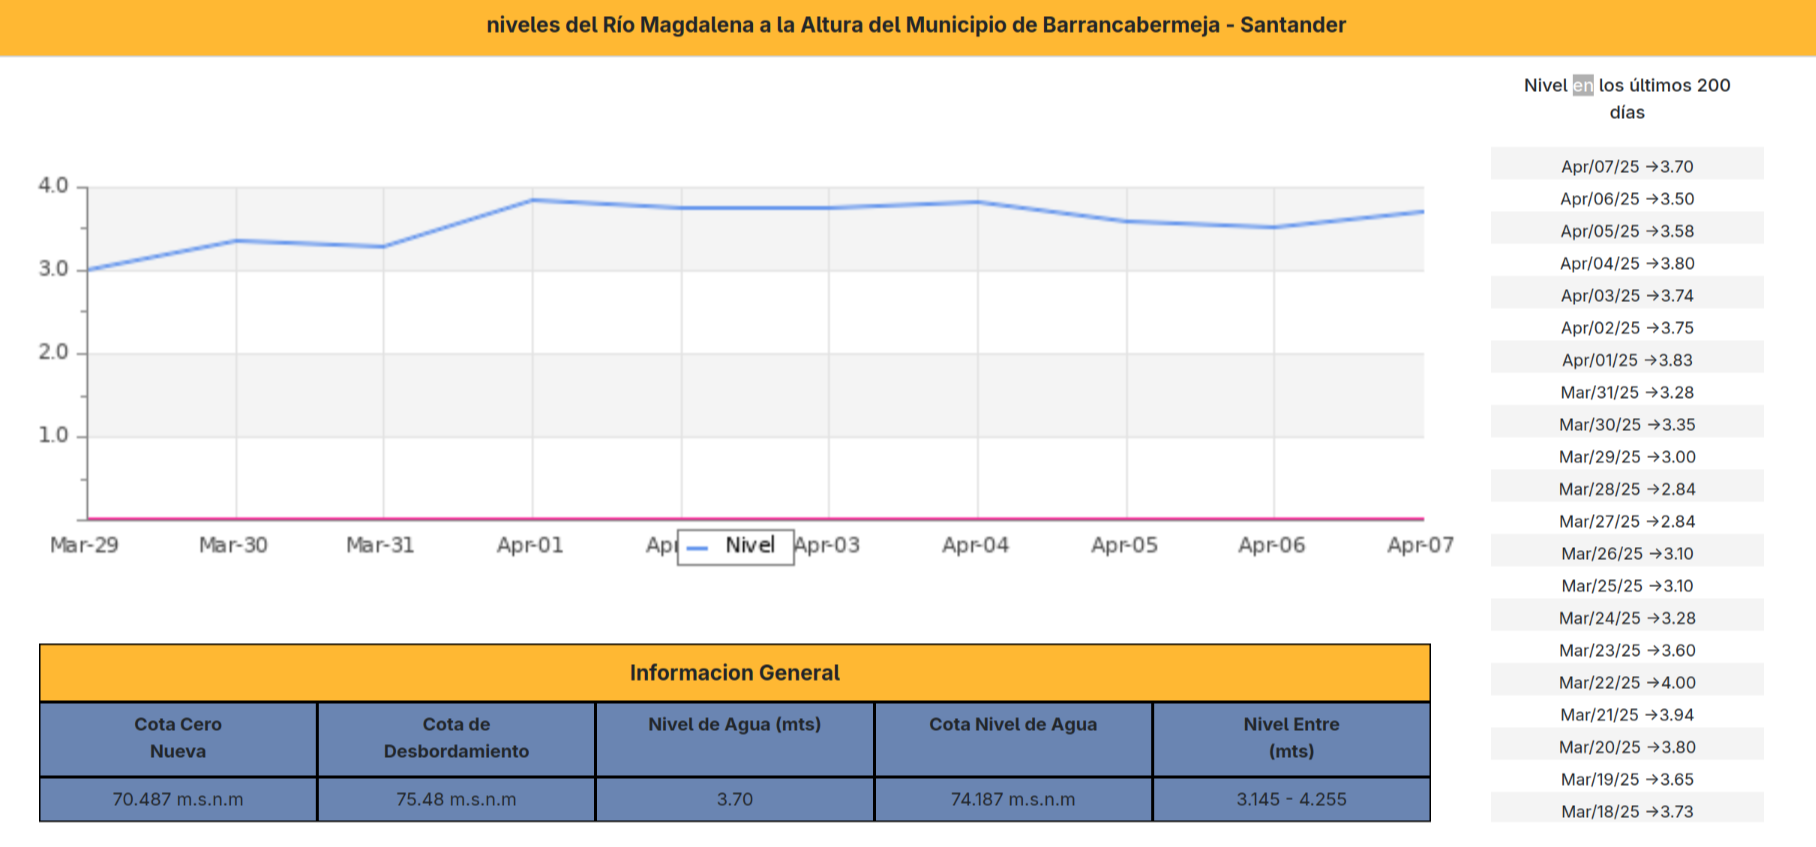
\includegraphics[width=1\textwidth]{img/Barran.png}
        \caption{Datos de CORMAGDALENA\cite{cormagdalena_niveles}}
      \end{figure}
    \end{column}
  \end{columns}

\end{frame}


\begin{frame}
  \frametitle{Datos históricos de caudal}

  \begin{columns}
    \begin{column}{.5\textwidth}
      \begin{itemize}
        \item Descarga del río Magdalena, datos desde julio de 1936 hasta agosto de 2024 
        \item Unidades en $m^{3}/s$.
        \item Toca hacer solicitud para descargar los datos.
      \end{itemize}
    \end{column}

    \begin{column}{.5\textwidth}
      \begin{figure}[ht]
        \centering
        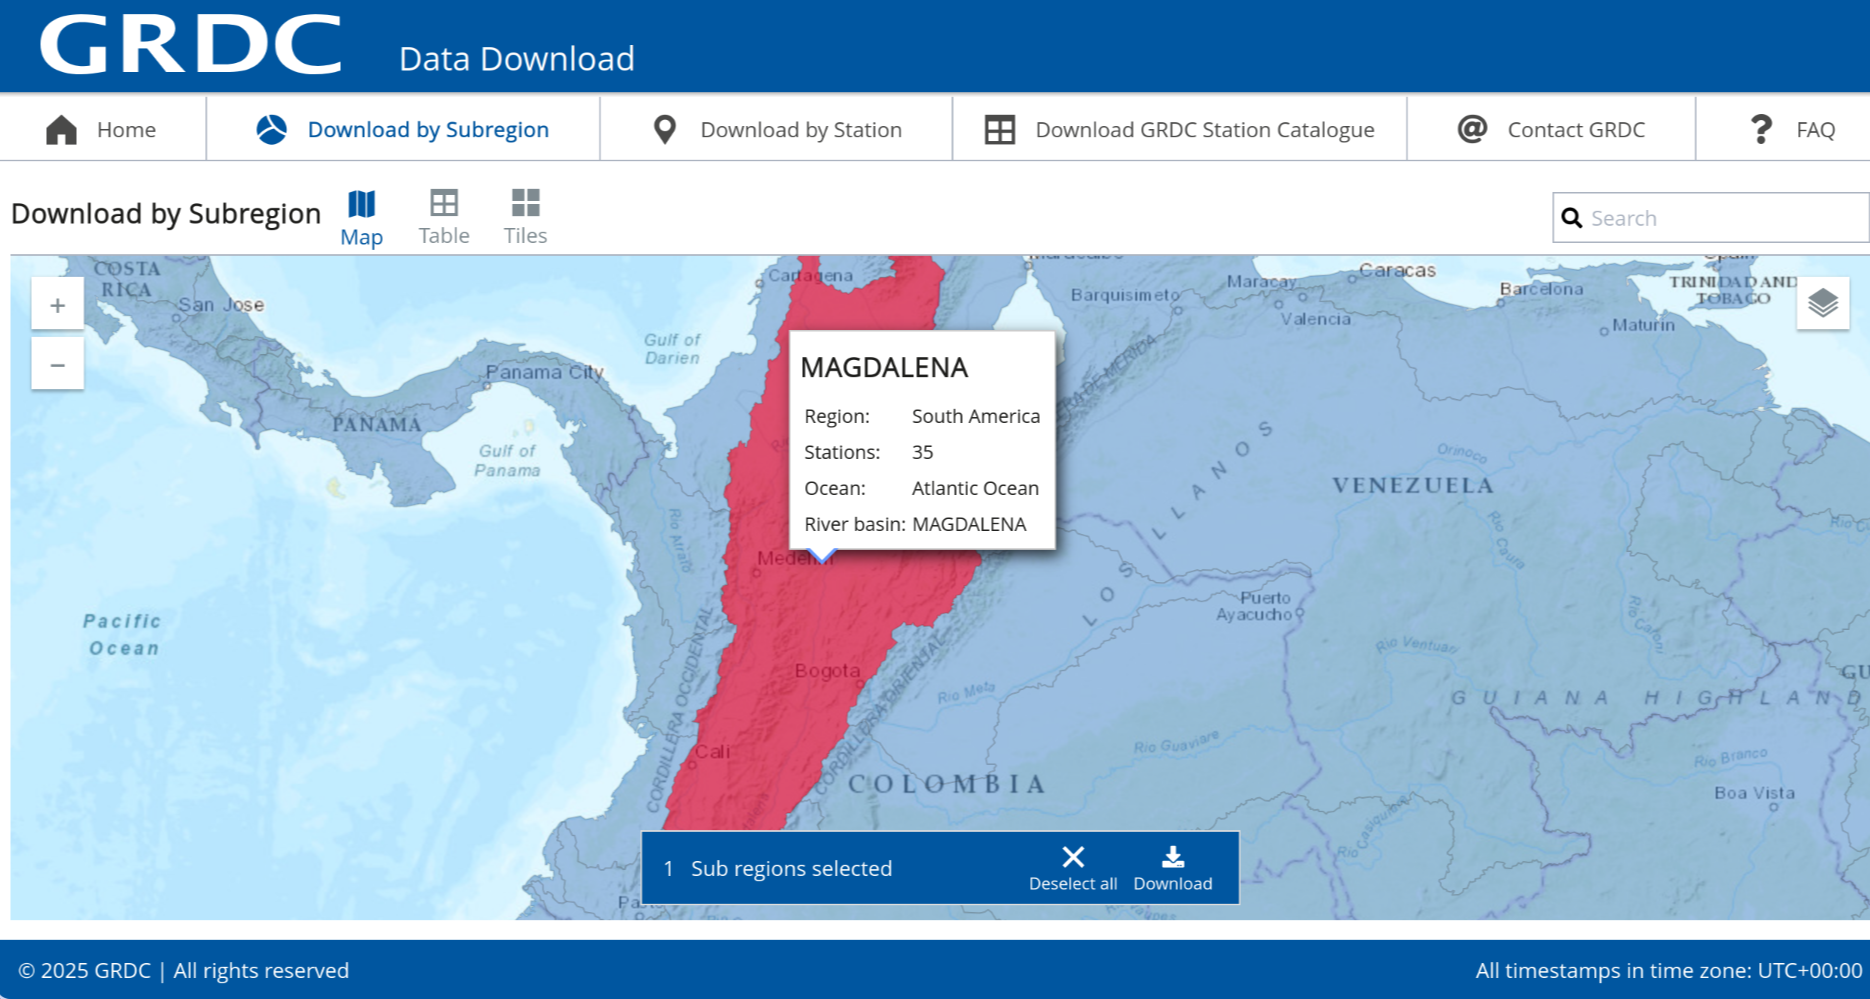
\includegraphics[width=1\textwidth]{img/GRDC.png}
        \caption{Portal de descarga del \textit{Global Runoff Data Center}\cite{grdc_data_portal}}
      \end{figure}
    \end{column}
  \end{columns}

\end{frame}


\section{Limpieza de datos}

\insertsectionpage

\begin{frame}[allowframebreaks]
  \frametitle{Limpieza datos de elevación del río}
      \begin{itemize}
        \item Según Cormagdalena\cite{cormagdalena_niveles} se registran niveles de la elevación en los últimos $~200$ días.
        \item Al realizar \lstinline!bat niveles.csv \| wc -l! da una salida de $1801$.
        \item Utilizando de la librería \textit{Pandas} y \textit{Python} se realiza una limpieza de duplicados y también una conversión de \textit{data type} a \textit{datetime}.
      \end{itemize}

      \newpage

      \begin{figure}[ht]
        \centering
        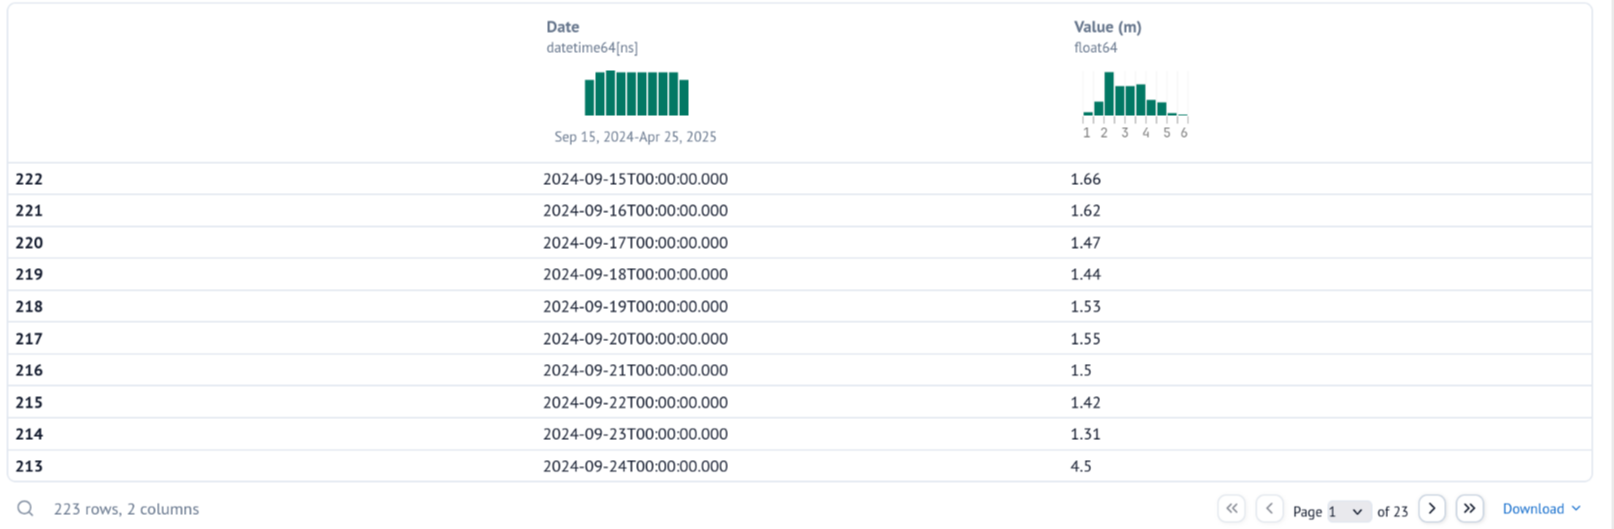
\includegraphics[width=\textwidth]{img/img1.png}
        \caption{Resultado de una celda en \textit{Marimo}, elaboración propia.}
      \end{figure}

\end{frame}

\begin{frame}[allowframebreaks]
  \frametitle{Limpieza datos del caudal}
\begin{columns}
  \begin{column}{.5\textwidth}
    \begin{itemize}
      \item Datos descargados del GRDC\cite{grdc_data_portal} y propiedad del Instituto de Hidrología, Metereología y Estudios Ambientales (IDEAM)\cite{ideam2025}.
      \item Datos desde enero de $1936$ hasta septiembre de $2024$.
      \item Formato ``YYYY-MM-DD;hh:mm; Value''.
    \end{itemize}
  \end{column}

  \begin{column}{.5\textwidth}
    \begin{figure}[ht]
      \centering
      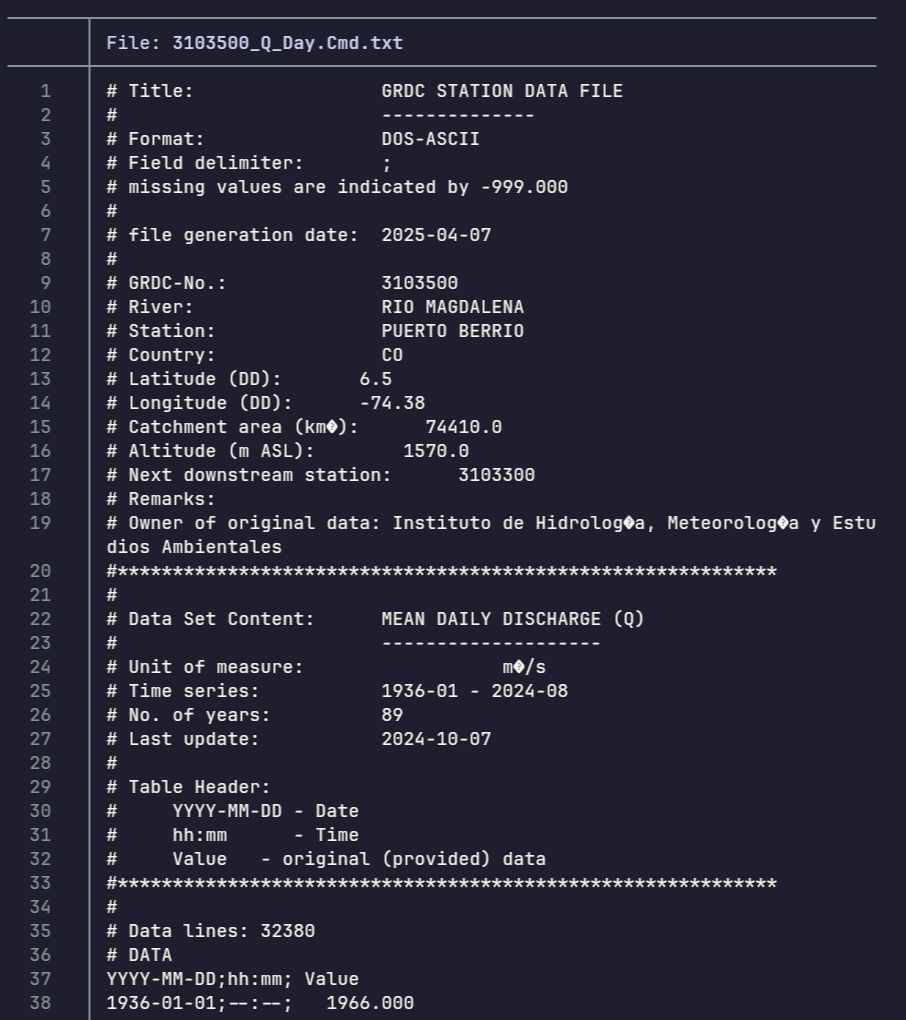
\includegraphics[width=0.6\textwidth]{img/img2.png}
    \end{figure}
  \end{column}

\end{columns}

\end{frame}

\newpage

\begin{columns}
  \begin{column}{.5\textwidth}
    \begin{itemize}
      \item Se utiliza la funcionalidad de \textit{pipelines} en UNIX para filtrar los datos.
      \item Se ejecuta \lstinline|tail -n +37 3103500_Q_Day.Cmd.txt \| cut -d ";" -f 1,3 \| head|
      \item Finalmente, se ejecuta \lstinline|tail -n +37 3103500_Q_Day.Cmd.txt \| cut -d ";" -f 1, 3 > Caudal.txt|
    \end{itemize}
  \end{column}

  \begin{column}{.5\textwidth}
    \begin{figure}[ht]
      \centering
      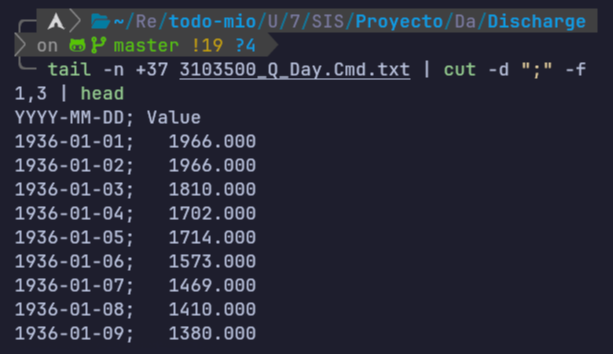
\includegraphics[width=\textwidth]{img/img3.png}
    \end{figure}

  \end{column}
\end{columns}

\newpage

\begin{columns}
  \begin{column}{.5\textwidth}
    \begin{itemize}
      \item Último dato registrado del caudal: $2024-08-25$.
      \item Primer dato registrado de la elevación del río: $2024-09-15$.
      \item Se toman períodos con variabilidad climática similar.
    \end{itemize}
  \end{column}

  \begin{column}{.5\textwidth}
\begin{figure}[ht]
  \centering
  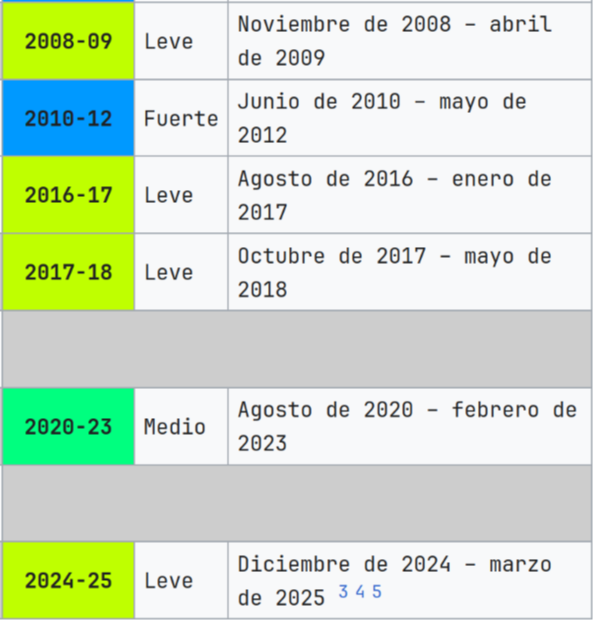
\includegraphics[width=0.5\textwidth]{img/img4.png}
  \caption{Sacado de \textit{Anexo:Eventos de El Niño y La Niña en el siglo XXI}\cite{eswiki:166933650}.}
\end{figure}

  \end{column}
\end{columns}



% \newpage 

% \begin{figure}[ht]
%   \centering
%   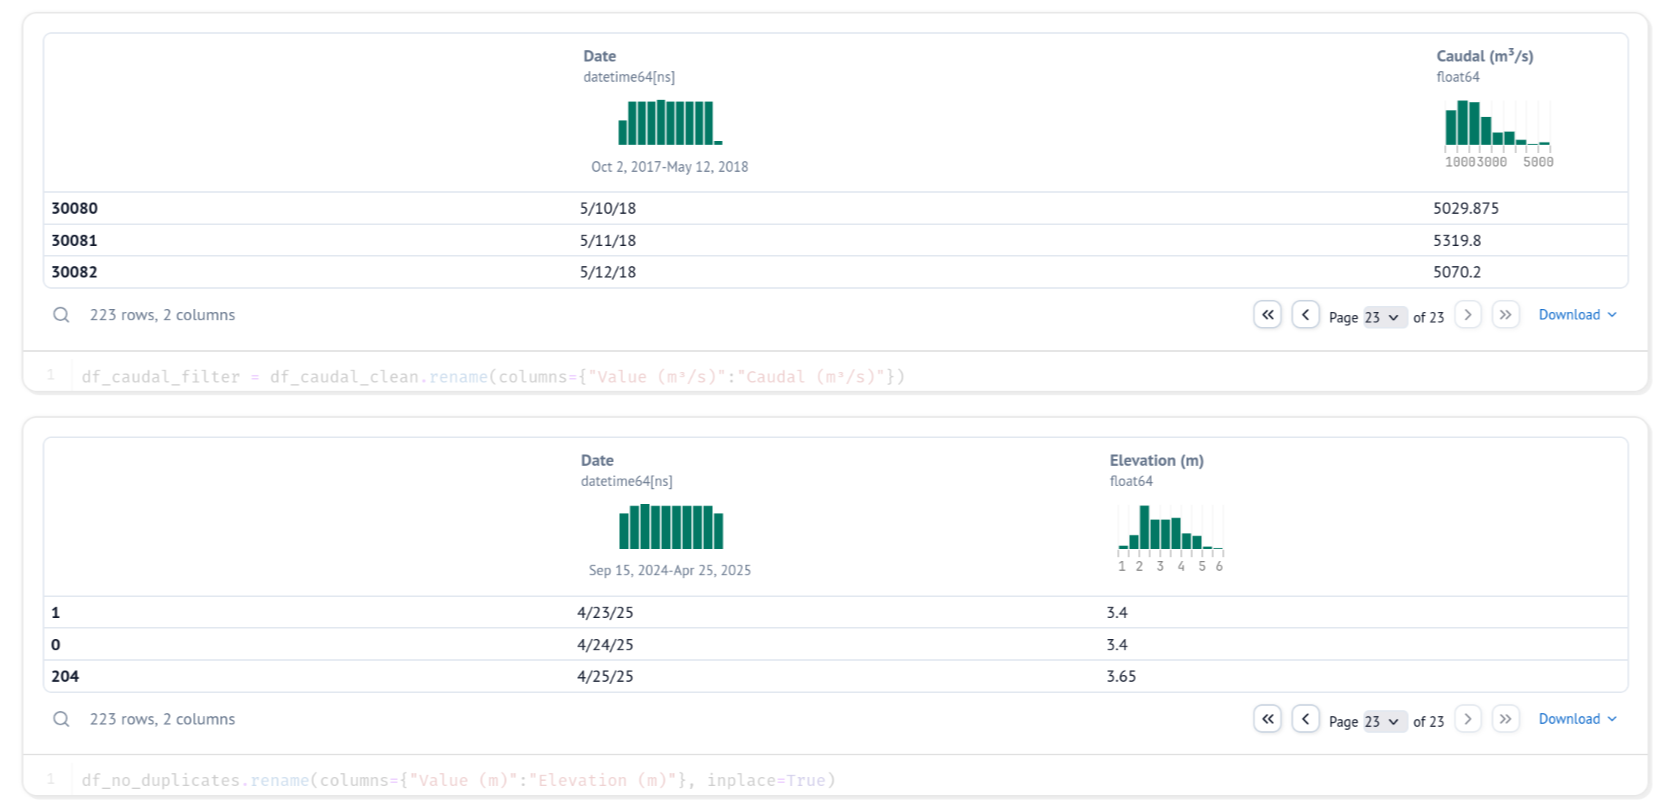
\includegraphics[width=0.7\textwidth]{img/img5.png}
%   \caption{Datos del caudal filtrados desde el 1 de octubre de 2017 y el 12 de mayo de 2018. El \textit{dataset} de la altura está completo. Elavoración propia usando \textit{Marimo}.}
% \end{figure}




\end{frame}




\section{Modelo matemático}

\insertsectionpage

\begin{frame}
  \frametitle{Ecuaciones de Saint-Venant - Ecuación de continuidad}
  \[
    \frac{\partial s_{c} (A + A_{0})}{\partial t} + \frac{\partial Q}{\partial x} - q_{L} = 0
  \]
  \begin{itemize}
    \item $s_{c}$ es el coeficiente de sinuosidad.
    \item $A$ es el área.
    \item $t$ es el tiempo.
    \item $Q$ es el cauldal.
    \item $x$ es la distancia del río.
    \item $q_{L}$ es el flujo lateral.
  \end{itemize}
\end{frame}

\begin{frame}
  \frametitle{Ecuaciones de Saint-Venant - Ecuación de continuidad}
  \[
  \frac{\partial S_{m}Q}{\partial t} + \frac{\partial (\beta Q^{2} / A) }{\partial x} + g A \left(\frac{\partial h_{r}}{\partial x} + S_{f} + S_{ec}  \right) + M_{L} = 0
  \]
  \begin{columns}
    \begin{column}{0.5\textwidth}
      \begin{itemize}
        \item $S_{m}$ es el factor de sinuosidad.
        \item $Q$ es el caudal.
        \item $t$ es el tiempo.
        \item $\beta$ es el coeficiente del momentum para la distribución de la velocidad.
        \item $A$ es el área.
        \item $x$ es la distancia del río.
      \end{itemize}
    \end{column}

    \begin{column}{0.5\textwidth}
      \begin{itemize}
        \item $g$ es la aceleración de la gravedad.
        \item $h_{r}$ es la altura del río.
        \item $S_{f}$ es la fricción de la pendiente.
        \item $S_{ec}$ es la pérdida por fricción.
        \item $M_{L}$ es el flujo del momento en los bordes.
      \end{itemize}
    \end{column}
  \end{columns}
\end{frame}

\begin{frame}
  \frametitle{Método de diferencias finitas - Ecuación de continuidad}

  \begin{align*}
  &\frac{\partial s_{c} (A + A_{0})}{\partial t} + \frac{\partial Q}{\partial x} - q_{L} = 0 \\
  &\frac{s_{c} (A + A_{0})_{i}^{j+1} - s_{c}(A + A_{0})_{i}^{j} }{\Delta t} + \frac{Q_{i}^{j} - Q_{i-1}^{j} }{\Delta x} - q_{Li}^{j} = 0   
\end{align*}

  \[
  A_{i}^{j+1} = \frac{\left(q_{Li}^{j} - \frac{Q_{i}^{j} - Q_{i-1}^{j} }{\Delta x}  \right) \Delta t + s_{c} (A + A_{0})_{i}^{j}}{s_{c}} - (A_{0})_{i}^{j+1}
  \]
  
\end{frame}


\begin{frame}
  \frametitle{Método de diferencias finitas - Ecuación de momentum}

  \begin{align*}
  \frac{s_{m} (Q)_{i}^{j+1} - s_{m}(Q)_{i}^{j} }{\Delta t} + \frac{(\beta Q^{2}/A)_{i}^{j} - (\beta Q^{2} /A)_{i-1}^{j} }{\Delta x} + gA \left( \frac{(h_{r})_{i}^{j} - (h_{r})_{i-1}^{j}}{\Delta x} + S_{f} + S_{ec}   \right) + M_{L} = 0   
\end{align*}

  \[
  Q_{i}^{j+1} = \frac{\left[ -M_{L} - g(A_{i}^{j}) \left(\frac{\left(\frac{A}{W}\right)_{i}^{j} - \left(\frac{A}{W}\right)_{i-1}^{j} }{\Delta x} + S_{t} + S_{a}  \right) - \frac{ \left( \frac{\beta Q^{2}}{A} \right)_{i}^{j} - \left( \frac{\beta Q^{2}}{A} \right)_{i-1}^{j}  }{\Delta x}           \right] \Delta t + S_{m} (Q)_{i}^{j}}{s_{m}}
  \]
  
  
\end{frame}

\section{Despliegue}

\insertsectionpage

\begin{frame}
  \frametitle{Despliegue}

  \begin{columns}
    \begin{column}{.5\textwidth}
      \begin{itemize}
        \item Tener experimentos locales en \textit{notebooks} está bien, pero... ¿Cómo pueden verse en internet? 
        \item Se realizó un despliegue en un servidor propio en Proxmox.
      \end{itemize}
    \end{column}

    \begin{column}{.5\textwidth}
      \begin{figure}[ht]
        \centering
        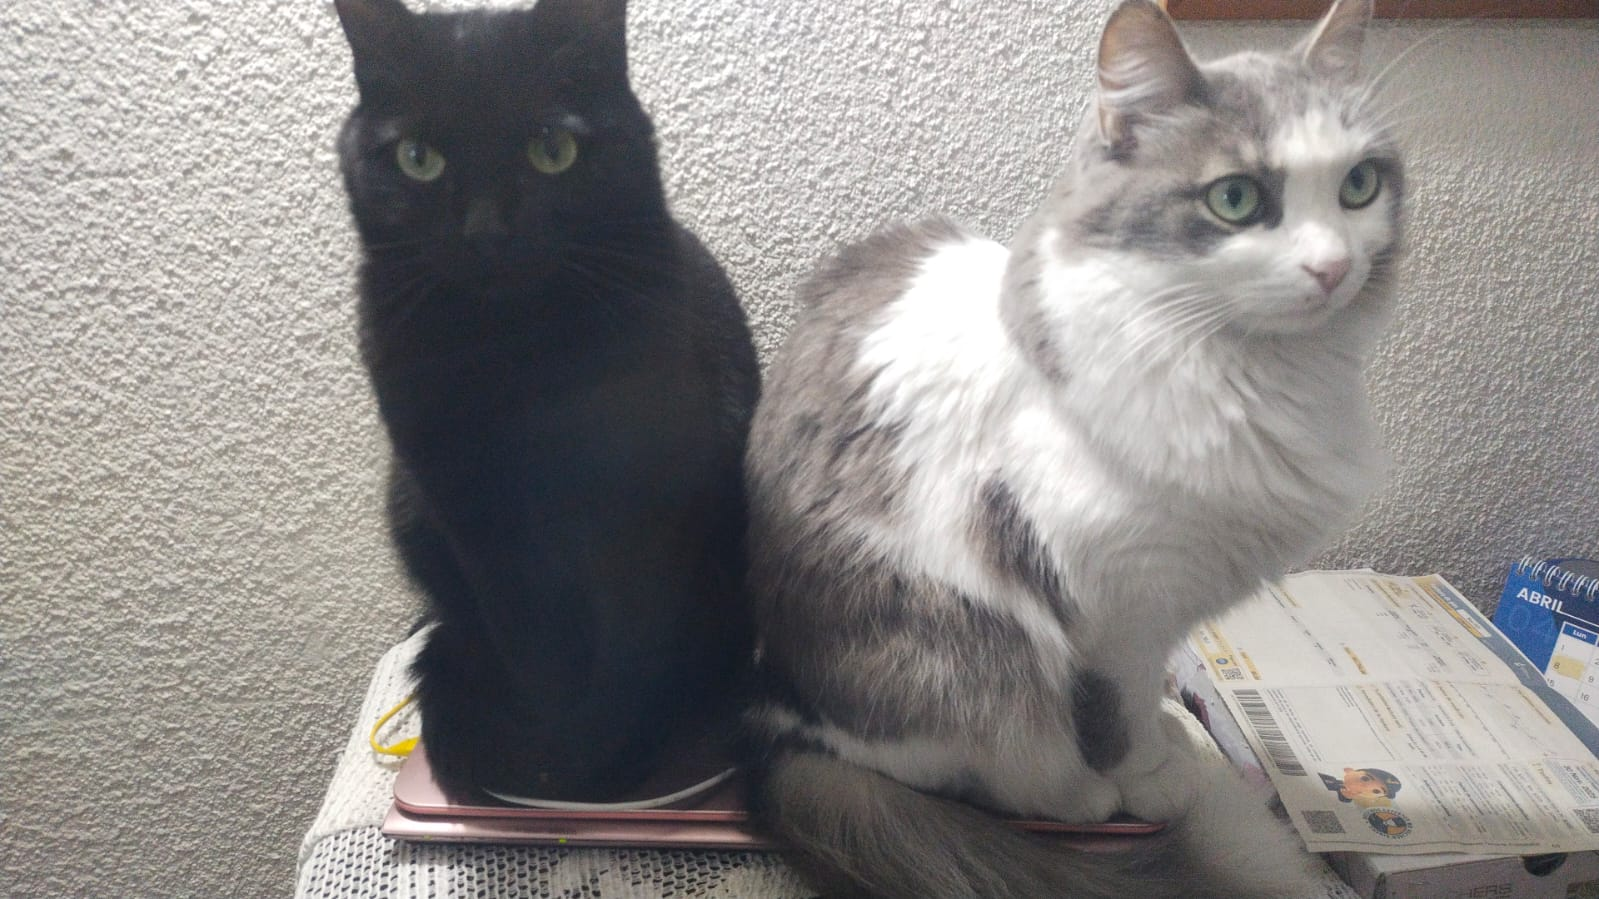
\includegraphics[width=0.8\textwidth]{img/Server1.jpg}
      \end{figure}

    \end{column}
  \end{columns}

\end{frame}

\begin{frame}
  \frametitle{Proxmox}

  \begin{columns}
    \begin{column}{.5\textwidth}
      \begin{itemize}
        \item Utilizando un computador viejo con menos de 4 de memoria RAM se obtiene un servidor para hacer virtualizaciones y despliegues con ayuda de Docker.
        \item Se tiene también el NGINX Proxy Manager encargado de recibir las direcciones y redireccionar al puerto indicado.
      \end{itemize}
    \end{column}

    \begin{column}{.5\textwidth}
      \begin{figure}[ht]
        \centering
        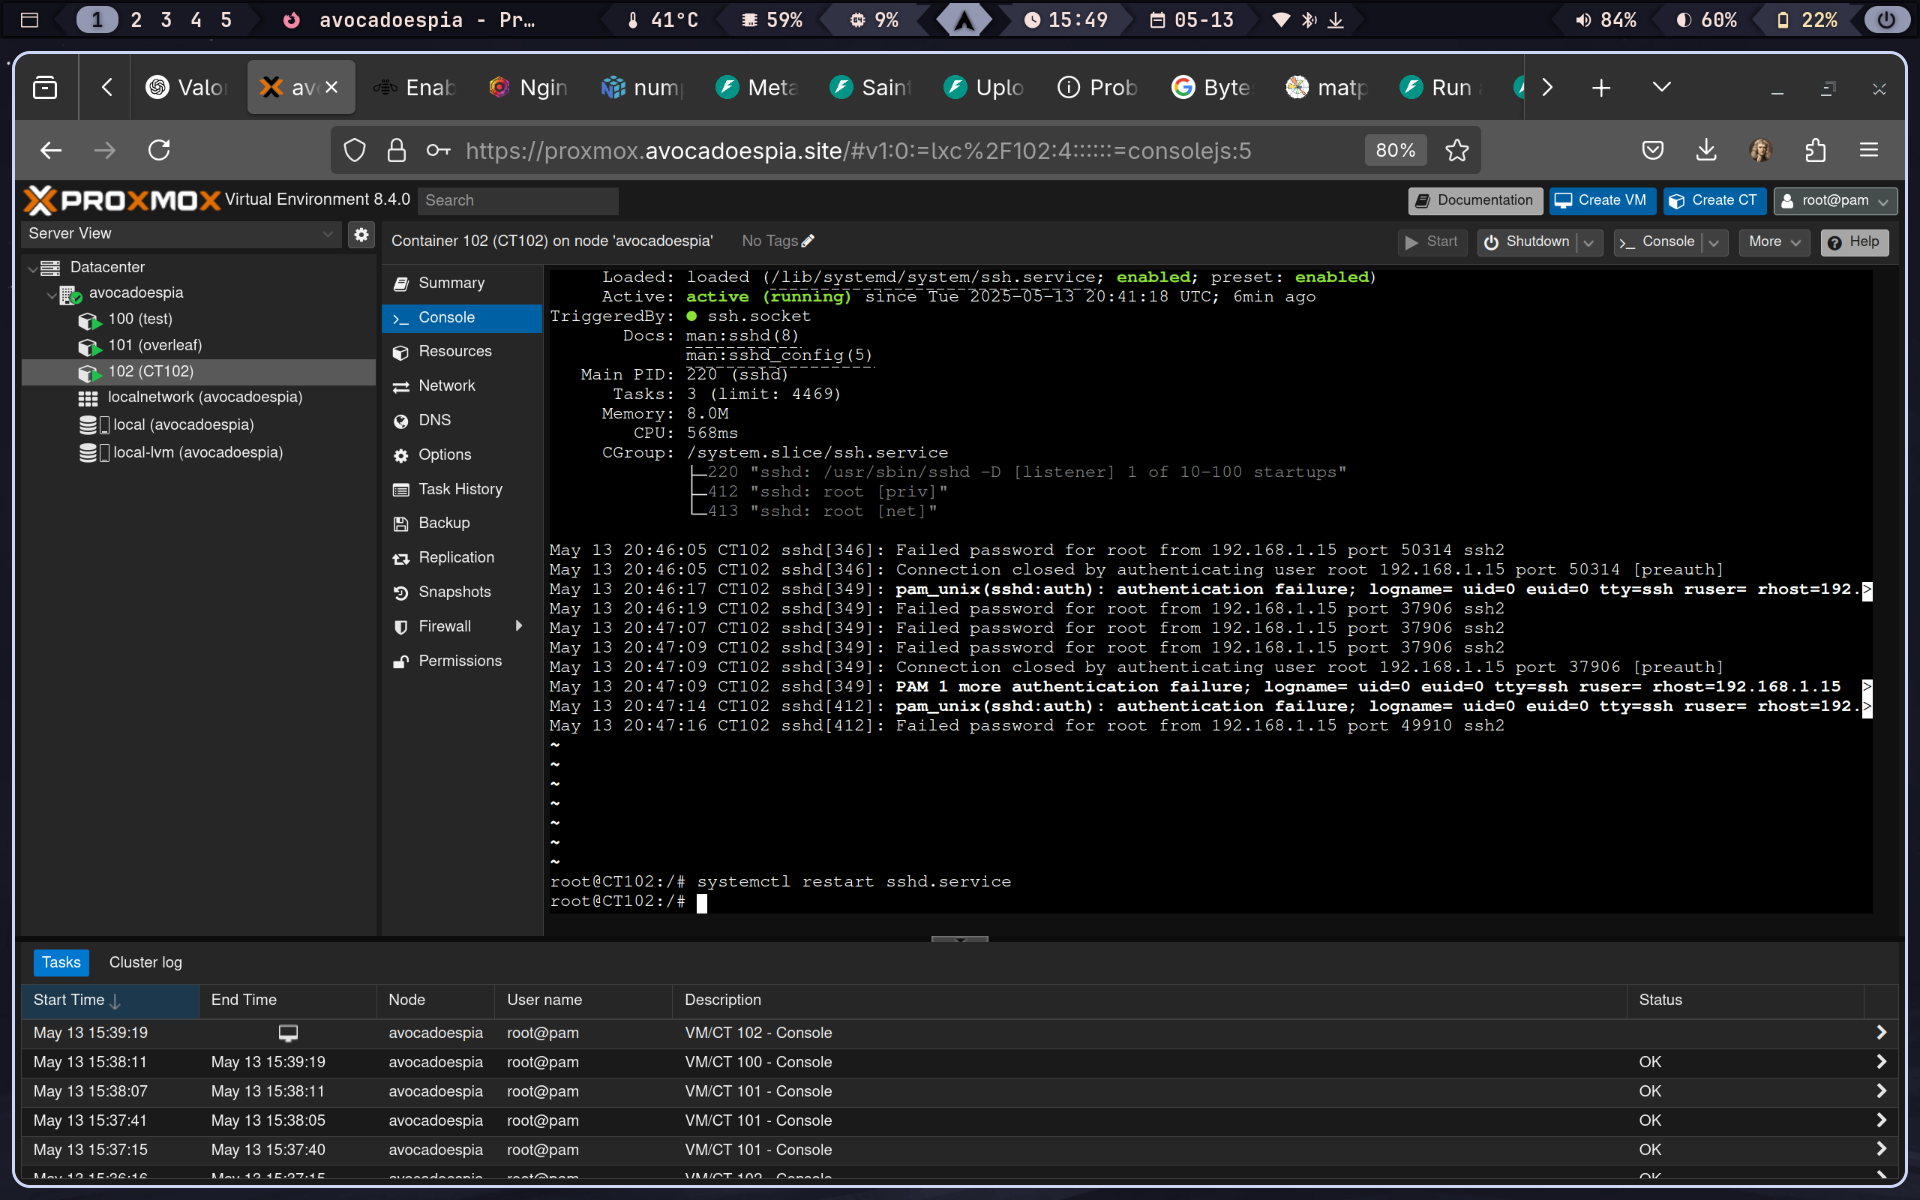
\includegraphics[width=0.8\textwidth]{img/Proxmox12.png}
      \end{figure}

    \end{column}
  \end{columns}

\end{frame}

\begin{frame}
  \frametitle{Docker}

  \begin{columns}
    \begin{column}{.5\textwidth}
      \begin{itemize}
        \item Se realizó un contenedor de Docker desplegado en un LXC y luego este se expone en un puerto. 
        \item El NGINX se encarga de remapear la dirección que llega por internet al contenedor en el servidor. 
      \end{itemize}
    \end{column}

    \begin{column}{.5\textwidth}
      \begin{figure}[ht]
        \centering
        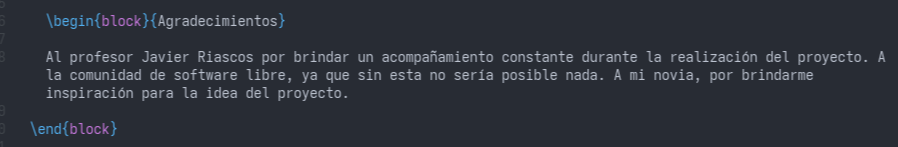
\includegraphics[width=0.8\textwidth]{img/Proxmox15.png}
      \end{figure}

    \end{column}
  \end{columns}

\end{frame}


\section{Licencia}

\insertsectionpage


\begin{frame}
  \frametitle{Licencia}

  \begin{columns}
    \begin{column}{.5\textwidth}
      \begin{itemize}
        \item Código, datos y contenido se encuentra en: \url{https://github.com/TheLudway/HydrologyDynamicsProject} 
        \item Todo bajo la licencia GPL V3 y CC BY SA 4.0 a excepción de los datos.
      \end{itemize}
    \end{column}

    \begin{column}{.5\textwidth}
      \begin{figure}[ht]
        \centering
        \href{https://www.gnu.org/licenses/gpl-3.0.txt}{\includesvg[width=0.8\textwidth]{img/GPL.svg}}
      \end{figure}
    \end{column}
  \end{columns}

\end{frame}


\section{Referencias}

\insertsectionpage
\begin{frame}[allowframebreaks]{Referencias}
  \printbibliography
\end{frame}


\insertendpage

\end{document}
